\documentclass[twoside]{book}

% Packages required by doxygen
\usepackage{fixltx2e}
\usepackage{calc}
\usepackage{doxygen}
\usepackage[export]{adjustbox} % also loads graphicx
\usepackage{graphicx}
\usepackage[utf8]{inputenc}
\usepackage{makeidx}
\usepackage{multicol}
\usepackage{multirow}
\PassOptionsToPackage{warn}{textcomp}
\usepackage{textcomp}
\usepackage[nointegrals]{wasysym}
\usepackage[table]{xcolor}

% Font selection
\usepackage[T1]{fontenc}
\usepackage[scaled=.90]{helvet}
\usepackage{courier}
\usepackage{amssymb}
\usepackage{sectsty}
\renewcommand{\familydefault}{\sfdefault}
\allsectionsfont{%
  \fontseries{bc}\selectfont%
  \color{darkgray}%
}
\renewcommand{\DoxyLabelFont}{%
  \fontseries{bc}\selectfont%
  \color{darkgray}%
}
\newcommand{\+}{\discretionary{\mbox{\scriptsize$\hookleftarrow$}}{}{}}

% Page & text layout
\usepackage{geometry}
\geometry{%
  a4paper,%
  top=2.5cm,%
  bottom=2.5cm,%
  left=2.5cm,%
  right=2.5cm%
}
\tolerance=750
\hfuzz=15pt
\hbadness=750
\setlength{\emergencystretch}{15pt}
\setlength{\parindent}{0cm}
\setlength{\parskip}{3ex plus 2ex minus 2ex}
\makeatletter
\renewcommand{\paragraph}{%
  \@startsection{paragraph}{4}{0ex}{-1.0ex}{1.0ex}{%
    \normalfont\normalsize\bfseries\SS@parafont%
  }%
}
\renewcommand{\subparagraph}{%
  \@startsection{subparagraph}{5}{0ex}{-1.0ex}{1.0ex}{%
    \normalfont\normalsize\bfseries\SS@subparafont%
  }%
}
\makeatother

% Headers & footers
\usepackage{fancyhdr}
\pagestyle{fancyplain}
\fancyhead[LE]{\fancyplain{}{\bfseries\thepage}}
\fancyhead[CE]{\fancyplain{}{}}
\fancyhead[RE]{\fancyplain{}{\bfseries\leftmark}}
\fancyhead[LO]{\fancyplain{}{\bfseries\rightmark}}
\fancyhead[CO]{\fancyplain{}{}}
\fancyhead[RO]{\fancyplain{}{\bfseries\thepage}}
\fancyfoot[LE]{\fancyplain{}{}}
\fancyfoot[CE]{\fancyplain{}{}}
\fancyfoot[RE]{\fancyplain{}{\bfseries\scriptsize Generated by Doxygen }}
\fancyfoot[LO]{\fancyplain{}{\bfseries\scriptsize Generated by Doxygen }}
\fancyfoot[CO]{\fancyplain{}{}}
\fancyfoot[RO]{\fancyplain{}{}}
\renewcommand{\footrulewidth}{0.4pt}
\renewcommand{\chaptermark}[1]{%
  \markboth{#1}{}%
}
\renewcommand{\sectionmark}[1]{%
  \markright{\thesection\ #1}%
}

% Indices & bibliography
\usepackage{natbib}
\usepackage[titles]{tocloft}
\setcounter{tocdepth}{3}
\setcounter{secnumdepth}{5}
\makeindex

% Hyperlinks (required, but should be loaded last)
\usepackage{ifpdf}
\ifpdf
  \usepackage[pdftex,pagebackref=true]{hyperref}
\else
  \usepackage[ps2pdf,pagebackref=true]{hyperref}
\fi
\hypersetup{%
  colorlinks=true,%
  linkcolor=blue,%
  citecolor=blue,%
  unicode%
}

% Custom commands
\newcommand{\clearemptydoublepage}{%
  \newpage{\pagestyle{empty}\cleardoublepage}%
}

\usepackage{caption}
\captionsetup{labelsep=space,justification=centering,font={bf},singlelinecheck=off,skip=4pt,position=top}

%===== C O N T E N T S =====

\begin{document}

% Titlepage & ToC
\hypersetup{pageanchor=false,
             bookmarksnumbered=true,
             pdfencoding=unicode
            }
\pagenumbering{alph}
\begin{titlepage}
\vspace*{7cm}
\begin{center}%
{\Large Simulador SE }\\
\vspace*{1cm}
{\large Generated by Doxygen 1.8.13}\\
\end{center}
\end{titlepage}
\clearemptydoublepage
\pagenumbering{roman}
\tableofcontents
\clearemptydoublepage
\pagenumbering{arabic}
\hypersetup{pageanchor=true}

%--- Begin generated contents ---
\chapter{Simulador Sistemas Embebidos Robotino}
\label{index}\hypertarget{index}{}\hypertarget{index_autotoc_md0}{}\section{Overview}\label{index_autotoc_md0}
Esta es la documentación del proyecto final de la catedra de Programación Orientada a Objetos en C++.\hypertarget{index_autotoc_md1}{}\section{Objetivos}\label{index_autotoc_md1}


El objetivo es simular la comunicación de 2 arduinos y una raspberry. Ademas, en la raspberry hay un thread corriendo que representa a una camara y envia datos de posición a la raspberry.\hypertarget{index_autotoc_md2}{}\section{Caracteristicas de los SE}\label{index_autotoc_md2}
\hypertarget{index_autotoc_md3}{}\subsection{Raspberry}\label{index_autotoc_md3}

\begin{DoxyItemize}
\item Intercambia mensajes con los Arduinos\+: Recibe mediciones de I\+MU y sensor de distancia y envia seteo de la bomba de agua.
\item Recibe datos del thread de la camara
\end{DoxyItemize}\hypertarget{index_autotoc_md4}{}\subsection{Arduino R}\label{index_autotoc_md4}

\begin{DoxyItemize}
\item Posee una I\+MU que mide aceleraciones en 3 ejes
\item Tiene conectada una bomba de agua a la cual se le setea la tensión
\end{DoxyItemize}\hypertarget{index_autotoc_md5}{}\subsection{Arduino L}\label{index_autotoc_md5}

\begin{DoxyItemize}
\item Tiene un sensor de posición laser
\end{DoxyItemize}\hypertarget{index_autotoc_md6}{}\section{Esquema del programa}\label{index_autotoc_md6}
El programa principal es el archivo \hyperlink{main_8cpp}{main.\+cpp}, donde se disparan los siguientes threads\+:
\begin{DoxyItemize}
\item AR\+: Corre el programa princiapl del Arduino R. En el se toman datos de una I\+MU y se envian a la raspberry. Ademas se leen mensajes que provienen de la raspberry para setear actuadores.
\item AL\+: Corre el programa principal del Arduino L. En el mismo se toman datos de un sensor de distancia y se envian a la raspberry
\item R\+PI\+: Corre el thread de la raspberry pi, dentro del cual se corren lo siguientes threads\+:
\begin{DoxyItemize}
\item Main\+: Corre el programa principal de la raspi, en el mismo se leen datos que provienen de los arduinos y se envian datos para setear los actuadores.
\item Camara\+: Lee datos de posición de la camara y los envia al programa principal de la raspi
\end{DoxyItemize}
\item Quit\+: Revisa si el usuario quiere terminar la simulacion (enter) en caso de querer terminar cierra todos los threads.
\end{DoxyItemize}

Para la generación de los datos de la I\+MU y la camara se leen archivos .txt con los datos de aceleración y posición. En el caso del sensor de distancia, se generan numeros aleatorios para representar la posición medida.\hypertarget{index_autotoc_md7}{}\section{Comunicaciones}\label{index_autotoc_md7}
Para simular la comunicación utilizo queue con strings como elementos donde voy metiendo los mensajes que quiero mandar a otros dispositivos, y el otro dispositivo lee si le corresponde y si le corresponde lo pop, sino no hace nada.

Las siguientes queue se utilizan\+:
\begin{DoxyItemize}
\item queue 1\+: Comunicación entre los arduinos y raspi
\item queue 2\+: Comunicación entre la raspi y la camara
\end{DoxyItemize}\hypertarget{index_autotoc_md8}{}\subsection{Envio de datos}\label{index_autotoc_md8}
A continuación se muestra la estructura de los mensajes de cada dispositivo. \subsubsection*{I\+MU}

!\+D\+AT\+:I\+M\+U\+:xxxx\+:yyyy\+:zzzz\+:\#

\subsubsection*{C\+A\+M\+E\+RA}

!\+D\+AT\+:C\+A\+M\+:xxxx\+:yyyy\+:zzzz\+:\#

\subsubsection*{L\+A\+S\+ER}

!\+D\+AT\+:L\+A\+S\+:xxxx\+:\# 
\chapter{Readme}
\label{md_src_Readme}
\Hypertarget{md_src_Readme}
\input{md_src_Readme}
\chapter{Hierarchical Index}
\section{Class Hierarchy}
This inheritance list is sorted roughly, but not completely, alphabetically\+:\begin{DoxyCompactList}
\item \contentsline{section}{Actuator}{\pageref{classActuator}}{}
\begin{DoxyCompactList}
\item \contentsline{section}{Jet\+Pump}{\pageref{classJetPump}}{}
\end{DoxyCompactList}
\item \contentsline{section}{Embeded\+System}{\pageref{classEmbededSystem}}{}
\begin{DoxyCompactList}
\item \contentsline{section}{ArduinoL}{\pageref{classArduinoL}}{}
\item \contentsline{section}{ArduinoR}{\pageref{classArduinoR}}{}
\item \contentsline{section}{Camera}{\pageref{classCamera}}{}
\item \contentsline{section}{Raspi}{\pageref{classRaspi}}{}
\end{DoxyCompactList}
\item \contentsline{section}{Message}{\pageref{classMessage}}{}
\begin{DoxyCompactList}
\item \contentsline{section}{Action\+Msg}{\pageref{classActionMsg}}{}
\item \contentsline{section}{Camera\+Msg}{\pageref{classCameraMsg}}{}
\item \contentsline{section}{Telemetry\+Msg}{\pageref{classTelemetryMsg}}{}
\end{DoxyCompactList}
\item \contentsline{section}{M\+P\+U9250}{\pageref{classMPU9250}}{}
\item \contentsline{section}{Sensor}{\pageref{classSensor}}{}
\begin{DoxyCompactList}
\item \contentsline{section}{Dist\+Sens}{\pageref{classDistSens}}{}
\end{DoxyCompactList}
\item \contentsline{section}{Timer}{\pageref{classTimer}}{}
\end{DoxyCompactList}

\chapter{Class Index}
\section{Class List}
Here are the classes, structs, unions and interfaces with brief descriptions\+:\begin{DoxyCompactList}
\item\contentsline{section}{\hyperlink{classhello}{hello} \\*Simple brief intro  detailed intro }{\pageref{classhello}}{}
\end{DoxyCompactList}

\chapter{File Index}
\section{File List}
Here is a list of all documented files with brief descriptions\+:\begin{DoxyCompactList}
\item\contentsline{section}{\hyperlink{main_8cpp}{main.\+cpp} }{\pageref{main_8cpp}}{}
\item\contentsline{section}{\hyperlink{robsim_8h}{robsim.\+h} }{\pageref{robsim_8h}}{}
\end{DoxyCompactList}

\chapter{Class Documentation}
\hypertarget{classActionMsg}{}\section{Action\+Msg Class Reference}
\label{classActionMsg}\index{Action\+Msg@{Action\+Msg}}


Clase mensaje de accion de control.  




{\ttfamily \#include $<$robsim.\+h$>$}



Inheritance diagram for Action\+Msg\+:\nopagebreak
\begin{figure}[H]
\begin{center}
\leavevmode
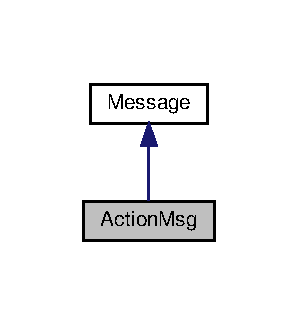
\includegraphics[width=143pt]{classActionMsg__inherit__graph}
\end{center}
\end{figure}


Collaboration diagram for Action\+Msg\+:\nopagebreak
\begin{figure}[H]
\begin{center}
\leavevmode
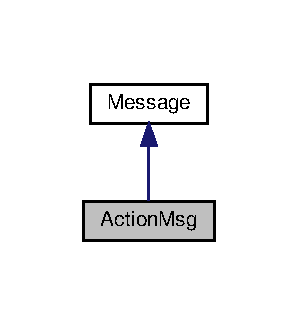
\includegraphics[width=143pt]{classActionMsg__coll__graph}
\end{center}
\end{figure}
\subsection*{Public Member Functions}
\begin{DoxyCompactItemize}
\item 
\hyperlink{classActionMsg_ab22c6cee704bd1ee2dbcbf54dd16cc4c}{Action\+Msg} ()
\end{DoxyCompactItemize}
\subsection*{Additional Inherited Members}


\subsection{Detailed Description}
Clase mensaje de accion de control. 

Definition at line 173 of file robsim.\+h.



\subsection{Constructor \& Destructor Documentation}
\mbox{\Hypertarget{classActionMsg_ab22c6cee704bd1ee2dbcbf54dd16cc4c}\label{classActionMsg_ab22c6cee704bd1ee2dbcbf54dd16cc4c}} 
\index{Action\+Msg@{Action\+Msg}!Action\+Msg@{Action\+Msg}}
\index{Action\+Msg@{Action\+Msg}!Action\+Msg@{Action\+Msg}}
\subsubsection{\texorpdfstring{Action\+Msg()}{ActionMsg()}}
{\footnotesize\ttfamily Action\+Msg\+::\+Action\+Msg (\begin{DoxyParamCaption}\item[{void}]{ }\end{DoxyParamCaption})}



Definition at line 110 of file robsim.\+cpp.



The documentation for this class was generated from the following files\+:\begin{DoxyCompactItemize}
\item 
src/\hyperlink{robsim_8h}{robsim.\+h}\item 
src/\hyperlink{robsim_8cpp}{robsim.\+cpp}\end{DoxyCompactItemize}

\hypertarget{classActuator}{}\section{Actuator Class Reference}
\label{classActuator}\index{Actuator@{Actuator}}


Clase base actuadores.  




{\ttfamily \#include $<$robsim.\+h$>$}



Inheritance diagram for Actuator\+:\nopagebreak
\begin{figure}[H]
\begin{center}
\leavevmode
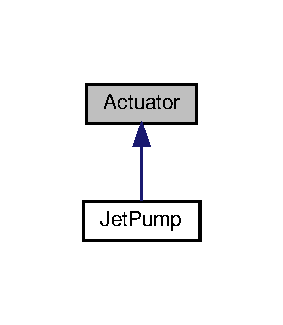
\includegraphics[width=136pt]{classActuator__inherit__graph}
\end{center}
\end{figure}


\subsection{Detailed Description}
Clase base actuadores. 

Definition at line 90 of file robsim.\+h.



The documentation for this class was generated from the following file\+:\begin{DoxyCompactItemize}
\item 
src/\hyperlink{robsim_8h}{robsim.\+h}\end{DoxyCompactItemize}

\hypertarget{classArduinoL}{}\section{ArduinoL Class Reference}
\label{classArduinoL}\index{ArduinoL@{ArduinoL}}


Clase que representa el Arduino dedicado al sistema 2 El metodo main es el bucle infinito del SE.  




{\ttfamily \#include $<$robsim.\+h$>$}



Inheritance diagram for ArduinoL\+:
\nopagebreak
\begin{figure}[H]
\begin{center}
\leavevmode
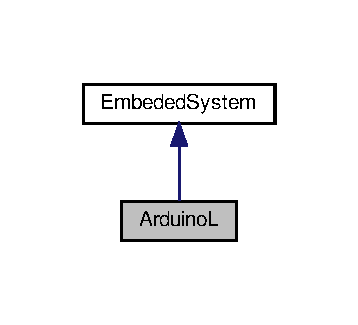
\includegraphics[width=172pt]{classArduinoL__inherit__graph}
\end{center}
\end{figure}


Collaboration diagram for ArduinoL\+:
\nopagebreak
\begin{figure}[H]
\begin{center}
\leavevmode
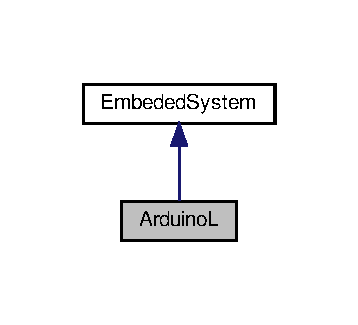
\includegraphics[width=172pt]{classArduinoL__coll__graph}
\end{center}
\end{figure}
\subsection*{Public Member Functions}
\begin{DoxyCompactItemize}
\item 
void \hyperlink{classArduinoL_a27a3e0f5bfbf48f558bce2d31a72d502}{main} ()
\begin{DoxyCompactList}\small\item\em Funcion virtual pura que corre el main del SE. \end{DoxyCompactList}\end{DoxyCompactItemize}


\subsection{Detailed Description}
Clase que representa el Arduino dedicado al sistema 2 El metodo main es el bucle infinito del SE. 

Definition at line 65 of file robsim.\+h.



\subsection{Member Function Documentation}
\mbox{\Hypertarget{classArduinoL_a27a3e0f5bfbf48f558bce2d31a72d502}\label{classArduinoL_a27a3e0f5bfbf48f558bce2d31a72d502}} 
\index{ArduinoL@{ArduinoL}!main@{main}}
\index{main@{main}!ArduinoL@{ArduinoL}}
\subsubsection{\texorpdfstring{main()}{main()}}
{\footnotesize\ttfamily void Arduino\+L\+::main (\begin{DoxyParamCaption}{ }\end{DoxyParamCaption})\hspace{0.3cm}{\ttfamily [virtual]}}



Funcion virtual pura que corre el main del SE. 



Implements \hyperlink{classEmbededSystem_a3a333d4954af4068f5e97301b4f55c48}{Embeded\+System}.



Definition at line 170 of file robsim.\+cpp.



The documentation for this class was generated from the following files\+:\begin{DoxyCompactItemize}
\item 
src/\hyperlink{robsim_8h}{robsim.\+h}\item 
src/\hyperlink{robsim_8cpp}{robsim.\+cpp}\end{DoxyCompactItemize}

\hypertarget{classArduinoR}{}\section{ArduinoR Class Reference}
\label{classArduinoR}\index{ArduinoR@{ArduinoR}}


Clase que representa el Arduino dedicado al sistema 1 El metodo main es el bucle infinito del SE Hereda de la clase Sistema Embebido.  




{\ttfamily \#include $<$robsim.\+h$>$}



Inheritance diagram for ArduinoR\+:
\nopagebreak
\begin{figure}[H]
\begin{center}
\leavevmode
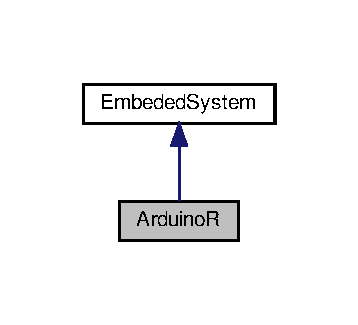
\includegraphics[width=172pt]{classArduinoR__inherit__graph}
\end{center}
\end{figure}


Collaboration diagram for ArduinoR\+:
\nopagebreak
\begin{figure}[H]
\begin{center}
\leavevmode
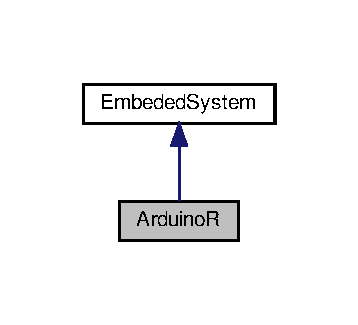
\includegraphics[width=172pt]{classArduinoR__coll__graph}
\end{center}
\end{figure}
\subsection*{Public Member Functions}
\begin{DoxyCompactItemize}
\item 
void \hyperlink{classArduinoR_a479b06fd9527e9810b37b91da8fb0f7e}{main} ()
\begin{DoxyCompactList}\small\item\em Funcion virtual pura que corre el main del SE. \end{DoxyCompactList}\item 
std\+::string \hyperlink{classArduinoR_a8365ffa8bde5c67337aa9b31fe08f83f}{read\+I\+MU} ()
\end{DoxyCompactItemize}


\subsection{Detailed Description}
Clase que representa el Arduino dedicado al sistema 1 El metodo main es el bucle infinito del SE Hereda de la clase Sistema Embebido. 

Definition at line 55 of file robsim.\+h.



\subsection{Member Function Documentation}
\mbox{\Hypertarget{classArduinoR_a479b06fd9527e9810b37b91da8fb0f7e}\label{classArduinoR_a479b06fd9527e9810b37b91da8fb0f7e}} 
\index{ArduinoR@{ArduinoR}!main@{main}}
\index{main@{main}!ArduinoR@{ArduinoR}}
\subsubsection{\texorpdfstring{main()}{main()}}
{\footnotesize\ttfamily void Arduino\+R\+::main (\begin{DoxyParamCaption}{ }\end{DoxyParamCaption})\hspace{0.3cm}{\ttfamily [virtual]}}



Funcion virtual pura que corre el main del SE. 



Implements \hyperlink{classEmbededSystem_a3a333d4954af4068f5e97301b4f55c48}{Embeded\+System}.



Definition at line 213 of file robsim.\+cpp.

\mbox{\Hypertarget{classArduinoR_a8365ffa8bde5c67337aa9b31fe08f83f}\label{classArduinoR_a8365ffa8bde5c67337aa9b31fe08f83f}} 
\index{ArduinoR@{ArduinoR}!read\+I\+MU@{read\+I\+MU}}
\index{read\+I\+MU@{read\+I\+MU}!ArduinoR@{ArduinoR}}
\subsubsection{\texorpdfstring{read\+I\+M\+U()}{readIMU()}}
{\footnotesize\ttfamily std\+::string Arduino\+R\+::read\+I\+MU (\begin{DoxyParamCaption}{ }\end{DoxyParamCaption})}



The documentation for this class was generated from the following files\+:\begin{DoxyCompactItemize}
\item 
src/\hyperlink{robsim_8h}{robsim.\+h}\item 
src/\hyperlink{robsim_8cpp}{robsim.\+cpp}\end{DoxyCompactItemize}

\hypertarget{classCamera}{}\section{Camera Class Reference}
\label{classCamera}\index{Camera@{Camera}}


Clase que representa la camara El metodo main es el bucle infinito del SE.  




{\ttfamily \#include $<$robsim.\+h$>$}



Inheritance diagram for Camera\+:\nopagebreak
\begin{figure}[H]
\begin{center}
\leavevmode
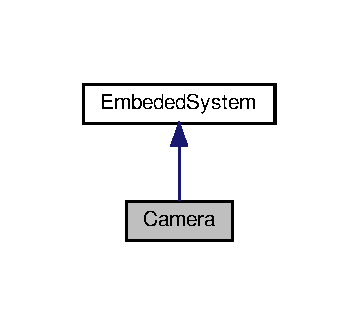
\includegraphics[width=172pt]{classCamera__inherit__graph}
\end{center}
\end{figure}


Collaboration diagram for Camera\+:\nopagebreak
\begin{figure}[H]
\begin{center}
\leavevmode
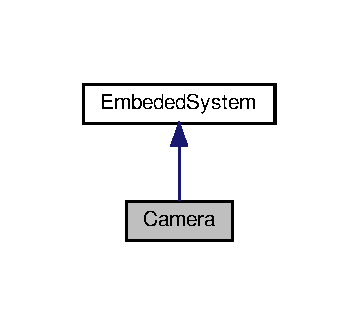
\includegraphics[width=172pt]{classCamera__coll__graph}
\end{center}
\end{figure}
\subsection*{Public Member Functions}
\begin{DoxyCompactItemize}
\item 
void \hyperlink{classCamera_a1719371e1e57ad18abfa5dd3d971bb39}{main} ()
\begin{DoxyCompactList}\small\item\em Funcion virtual pura que corre el main del SE. \end{DoxyCompactList}\end{DoxyCompactItemize}


\subsection{Detailed Description}
Clase que representa la camara El metodo main es el bucle infinito del SE. 

Definition at line 82 of file robsim.\+h.



\subsection{Member Function Documentation}
\mbox{\Hypertarget{classCamera_a1719371e1e57ad18abfa5dd3d971bb39}\label{classCamera_a1719371e1e57ad18abfa5dd3d971bb39}} 
\index{Camera@{Camera}!main@{main}}
\index{main@{main}!Camera@{Camera}}
\subsubsection{\texorpdfstring{main()}{main()}}
{\footnotesize\ttfamily void Camera\+::main (\begin{DoxyParamCaption}{ }\end{DoxyParamCaption})\hspace{0.3cm}{\ttfamily [virtual]}}



Funcion virtual pura que corre el main del SE. 



Implements \hyperlink{classEmbededSystem_a3a333d4954af4068f5e97301b4f55c48}{Embeded\+System}.



Definition at line 137 of file robsim.\+cpp.



The documentation for this class was generated from the following files\+:\begin{DoxyCompactItemize}
\item 
src/\hyperlink{robsim_8h}{robsim.\+h}\item 
src/\hyperlink{robsim_8cpp}{robsim.\+cpp}\end{DoxyCompactItemize}

\hypertarget{classCameraMsg}{}\section{Camera\+Msg Class Reference}
\label{classCameraMsg}\index{Camera\+Msg@{Camera\+Msg}}


Clase mensaje de camara.  




{\ttfamily \#include $<$robsim.\+h$>$}



Inheritance diagram for Camera\+Msg\+:\nopagebreak
\begin{figure}[H]
\begin{center}
\leavevmode
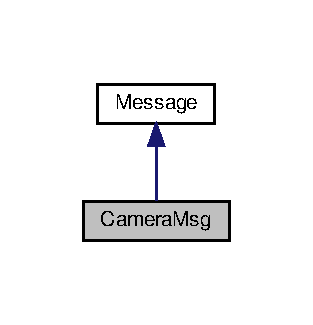
\includegraphics[width=150pt]{classCameraMsg__inherit__graph}
\end{center}
\end{figure}


Collaboration diagram for Camera\+Msg\+:\nopagebreak
\begin{figure}[H]
\begin{center}
\leavevmode
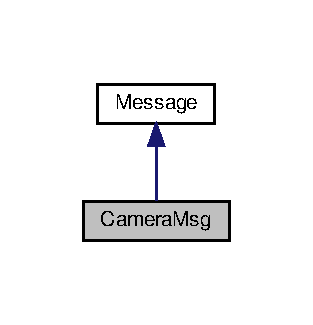
\includegraphics[width=150pt]{classCameraMsg__coll__graph}
\end{center}
\end{figure}
\subsection*{Public Member Functions}
\begin{DoxyCompactItemize}
\item 
\hyperlink{classCameraMsg_a5c60f7195b2abc7fdbd2c4568c8708d4}{Camera\+Msg} ()
\item 
void \hyperlink{classCameraMsg_a533eef67ac13dabdb81969eff6aaa267}{write\+\_\+pos} (double camX, double camY, double camZ)
\begin{DoxyCompactList}\small\item\em Metodo que recibe los valores de posicion y lo escribe en un msj (atributo de clase base. \end{DoxyCompactList}\end{DoxyCompactItemize}
\subsection*{Additional Inherited Members}


\subsection{Detailed Description}
Clase mensaje de camara. 

Definition at line 182 of file robsim.\+h.



\subsection{Constructor \& Destructor Documentation}
\mbox{\Hypertarget{classCameraMsg_a5c60f7195b2abc7fdbd2c4568c8708d4}\label{classCameraMsg_a5c60f7195b2abc7fdbd2c4568c8708d4}} 
\index{Camera\+Msg@{Camera\+Msg}!Camera\+Msg@{Camera\+Msg}}
\index{Camera\+Msg@{Camera\+Msg}!Camera\+Msg@{Camera\+Msg}}
\subsubsection{\texorpdfstring{Camera\+Msg()}{CameraMsg()}}
{\footnotesize\ttfamily Camera\+Msg\+::\+Camera\+Msg (\begin{DoxyParamCaption}\item[{void}]{ }\end{DoxyParamCaption})}



Definition at line 115 of file robsim.\+cpp.



\subsection{Member Function Documentation}
\mbox{\Hypertarget{classCameraMsg_a533eef67ac13dabdb81969eff6aaa267}\label{classCameraMsg_a533eef67ac13dabdb81969eff6aaa267}} 
\index{Camera\+Msg@{Camera\+Msg}!write\+\_\+pos@{write\+\_\+pos}}
\index{write\+\_\+pos@{write\+\_\+pos}!Camera\+Msg@{Camera\+Msg}}
\subsubsection{\texorpdfstring{write\+\_\+pos()}{write\_pos()}}
{\footnotesize\ttfamily void Camera\+Msg\+::write\+\_\+pos (\begin{DoxyParamCaption}\item[{double}]{camX,  }\item[{double}]{camY,  }\item[{double}]{camZ }\end{DoxyParamCaption})}



Metodo que recibe los valores de posicion y lo escribe en un msj (atributo de clase base. 


\begin{DoxyParams}[1]{Parameters}
\mbox{\tt in}  & {\em camX} & Posición en x medida por la camara \\
\hline
\mbox{\tt in}  & {\em camY} & Posición en y medida por la camara \\
\hline
\mbox{\tt in}  & {\em camZ} & Posición en z medida por la camara \\
\hline
\end{DoxyParams}


Definition at line 120 of file robsim.\+cpp.



The documentation for this class was generated from the following files\+:\begin{DoxyCompactItemize}
\item 
src/\hyperlink{robsim_8h}{robsim.\+h}\item 
src/\hyperlink{robsim_8cpp}{robsim.\+cpp}\end{DoxyCompactItemize}

\hypertarget{classDistSens}{}\section{Dist\+Sens Class Reference}
\label{classDistSens}\index{Dist\+Sens@{Dist\+Sens}}


Clase que representa el sensor de dist.  




{\ttfamily \#include $<$robsim.\+h$>$}



Inheritance diagram for Dist\+Sens\+:\nopagebreak
\begin{figure}[H]
\begin{center}
\leavevmode
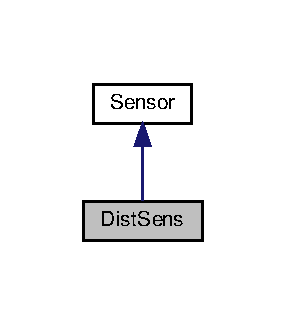
\includegraphics[width=137pt]{classDistSens__inherit__graph}
\end{center}
\end{figure}


Collaboration diagram for Dist\+Sens\+:\nopagebreak
\begin{figure}[H]
\begin{center}
\leavevmode
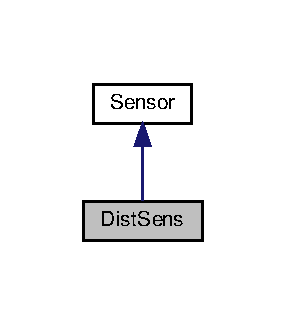
\includegraphics[width=137pt]{classDistSens__coll__graph}
\end{center}
\end{figure}


\subsection{Detailed Description}
Clase que representa el sensor de dist. 

Definition at line 133 of file robsim.\+h.



The documentation for this class was generated from the following file\+:\begin{DoxyCompactItemize}
\item 
src/\hyperlink{robsim_8h}{robsim.\+h}\end{DoxyCompactItemize}

\hypertarget{classEmbededSystem}{}\section{Embeded\+System Class Reference}
\label{classEmbededSystem}\index{Embeded\+System@{Embeded\+System}}


a Clase base Sistema embebido Tiene como metodo virtual puro el main de los SE  




{\ttfamily \#include $<$robsim.\+h$>$}



Inheritance diagram for Embeded\+System\+:
\nopagebreak
\begin{figure}[H]
\begin{center}
\leavevmode
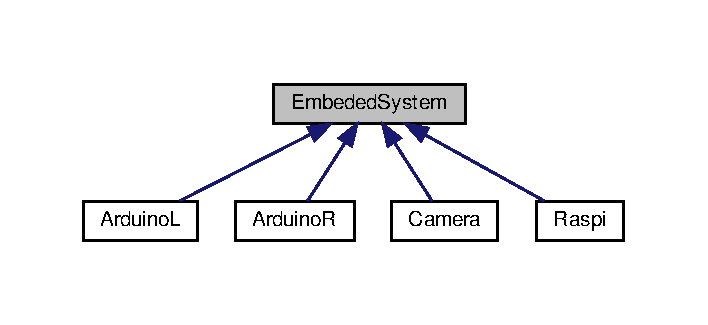
\includegraphics[width=340pt]{classEmbededSystem__inherit__graph}
\end{center}
\end{figure}
\subsection*{Public Member Functions}
\begin{DoxyCompactItemize}
\item 
virtual void \hyperlink{classEmbededSystem_a3a333d4954af4068f5e97301b4f55c48}{main} ()=0
\begin{DoxyCompactList}\small\item\em Funcion virtual pura que corre el main del SE. \end{DoxyCompactList}\end{DoxyCompactItemize}


\subsection{Detailed Description}
a Clase base Sistema embebido Tiene como metodo virtual puro el main de los SE 

Definition at line 44 of file robsim.\+h.



\subsection{Member Function Documentation}
\mbox{\Hypertarget{classEmbededSystem_a3a333d4954af4068f5e97301b4f55c48}\label{classEmbededSystem_a3a333d4954af4068f5e97301b4f55c48}} 
\index{Embeded\+System@{Embeded\+System}!main@{main}}
\index{main@{main}!Embeded\+System@{Embeded\+System}}
\subsubsection{\texorpdfstring{main()}{main()}}
{\footnotesize\ttfamily virtual void Embeded\+System\+::main (\begin{DoxyParamCaption}{ }\end{DoxyParamCaption})\hspace{0.3cm}{\ttfamily [pure virtual]}}



Funcion virtual pura que corre el main del SE. 



Implemented in \hyperlink{classCamera_a1719371e1e57ad18abfa5dd3d971bb39}{Camera}, \hyperlink{classRaspi_adce86197732891370a63b239cc413c7e}{Raspi}, \hyperlink{classArduinoL_a27a3e0f5bfbf48f558bce2d31a72d502}{ArduinoL}, and \hyperlink{classArduinoR_a479b06fd9527e9810b37b91da8fb0f7e}{ArduinoR}.



The documentation for this class was generated from the following file\+:\begin{DoxyCompactItemize}
\item 
src/\hyperlink{robsim_8h}{robsim.\+h}\end{DoxyCompactItemize}

\hypertarget{classJetPump}{}\section{Jet\+Pump Class Reference}
\label{classJetPump}\index{Jet\+Pump@{Jet\+Pump}}


Clase \hyperlink{classJetPump}{Jet\+Pump}.  




{\ttfamily \#include $<$robsim.\+h$>$}



Inheritance diagram for Jet\+Pump\+:\nopagebreak
\begin{figure}[H]
\begin{center}
\leavevmode
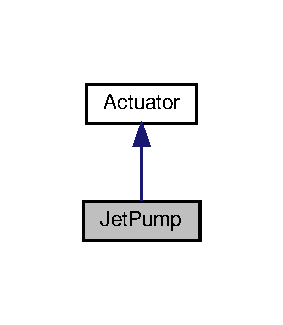
\includegraphics[width=136pt]{classJetPump__inherit__graph}
\end{center}
\end{figure}


Collaboration diagram for Jet\+Pump\+:\nopagebreak
\begin{figure}[H]
\begin{center}
\leavevmode
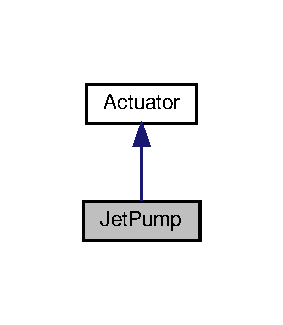
\includegraphics[width=136pt]{classJetPump__coll__graph}
\end{center}
\end{figure}
\subsection*{Public Member Functions}
\begin{DoxyCompactItemize}
\item 
\hyperlink{classJetPump_af259fad2aee62387e353b9911c8bb294}{Jet\+Pump} ()
\begin{DoxyCompactList}\small\item\em Constructor por defecto pone la tensión de la bomba en 0. \end{DoxyCompactList}\item 
void \hyperlink{classJetPump_ab817ef3e43d409ffbce2b72583866000}{set} (double V\+\_\+)
\begin{DoxyCompactList}\small\item\em Función que setea el valor de tensión de la bomba. \end{DoxyCompactList}\item 
double \hyperlink{classJetPump_adb125b513288b6783cc27fce155a6cb5}{get} ()
\begin{DoxyCompactList}\small\item\em Función que retorna el valor de la tensión actual de la bomba. \end{DoxyCompactList}\end{DoxyCompactItemize}


\subsection{Detailed Description}
Clase \hyperlink{classJetPump}{Jet\+Pump}. 

Representa una bombita del robot Tiene como atributo la tensión en bornes de la bomba y metodos que permiten setear y leer este valor 

Definition at line 106 of file robsim.\+h.



\subsection{Constructor \& Destructor Documentation}
\mbox{\Hypertarget{classJetPump_af259fad2aee62387e353b9911c8bb294}\label{classJetPump_af259fad2aee62387e353b9911c8bb294}} 
\index{Jet\+Pump@{Jet\+Pump}!Jet\+Pump@{Jet\+Pump}}
\index{Jet\+Pump@{Jet\+Pump}!Jet\+Pump@{Jet\+Pump}}
\subsubsection{\texorpdfstring{Jet\+Pump()}{JetPump()}}
{\footnotesize\ttfamily Jet\+Pump\+::\+Jet\+Pump (\begin{DoxyParamCaption}{ }\end{DoxyParamCaption})\hspace{0.3cm}{\ttfamily [inline]}}



Constructor por defecto pone la tensión de la bomba en 0. 



Definition at line 108 of file robsim.\+h.



\subsection{Member Function Documentation}
\mbox{\Hypertarget{classJetPump_adb125b513288b6783cc27fce155a6cb5}\label{classJetPump_adb125b513288b6783cc27fce155a6cb5}} 
\index{Jet\+Pump@{Jet\+Pump}!get@{get}}
\index{get@{get}!Jet\+Pump@{Jet\+Pump}}
\subsubsection{\texorpdfstring{get()}{get()}}
{\footnotesize\ttfamily double Jet\+Pump\+::get (\begin{DoxyParamCaption}{ }\end{DoxyParamCaption})\hspace{0.3cm}{\ttfamily [inline]}}



Función que retorna el valor de la tensión actual de la bomba. 

\begin{DoxyReturn}{Returns}
Tensión en la bomba 
\end{DoxyReturn}


Definition at line 119 of file robsim.\+h.

\mbox{\Hypertarget{classJetPump_ab817ef3e43d409ffbce2b72583866000}\label{classJetPump_ab817ef3e43d409ffbce2b72583866000}} 
\index{Jet\+Pump@{Jet\+Pump}!set@{set}}
\index{set@{set}!Jet\+Pump@{Jet\+Pump}}
\subsubsection{\texorpdfstring{set()}{set()}}
{\footnotesize\ttfamily void Jet\+Pump\+::set (\begin{DoxyParamCaption}\item[{double}]{V\+\_\+ }\end{DoxyParamCaption})\hspace{0.3cm}{\ttfamily [inline]}}



Función que setea el valor de tensión de la bomba. 


\begin{DoxyParams}[1]{Parameters}
\mbox{\tt in}  & {\em V\+\_\+} & Tensión que quiero colocar en la bomba \\
\hline
\end{DoxyParams}


Definition at line 113 of file robsim.\+h.



The documentation for this class was generated from the following file\+:\begin{DoxyCompactItemize}
\item 
src/\hyperlink{robsim_8h}{robsim.\+h}\end{DoxyCompactItemize}

\hypertarget{classMessage}{}\section{Message Class Reference}
\label{classMessage}\index{Message@{Message}}


Clase Mensaje.  




{\ttfamily \#include $<$robsim.\+h$>$}



Inheritance diagram for Message\+:\nopagebreak
\begin{figure}[H]
\begin{center}
\leavevmode
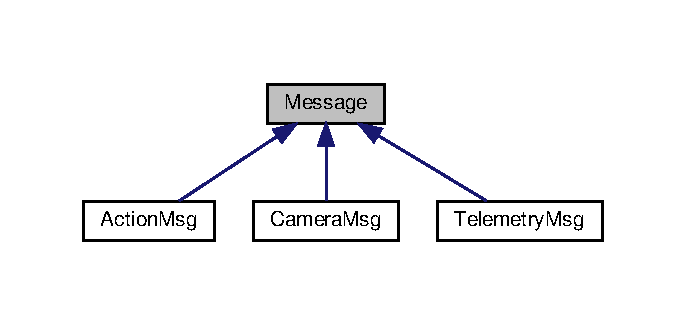
\includegraphics[width=329pt]{classMessage__inherit__graph}
\end{center}
\end{figure}
\subsection*{Public Types}
\begin{DoxyCompactItemize}
\item 
enum \hyperlink{classMessage_a1c65ab3f02ba5b175f583f9d275ecf2b}{Type} \{ \hyperlink{classMessage_a1c65ab3f02ba5b175f583f9d275ecf2babb3d2d909c73fe49800949a344775f8b}{Type\+::\+T\+E\+L\+E\+M\+E\+T\+RY}, 
\hyperlink{classMessage_a1c65ab3f02ba5b175f583f9d275ecf2bae58a1b00942e66d8b4abc960da7877ab}{Type\+::\+A\+C\+T\+I\+ON}, 
\hyperlink{classMessage_a1c65ab3f02ba5b175f583f9d275ecf2baddf0d6b21537d984fea6544f58101fa8}{Type\+::\+C\+A\+M\+E\+RA}
 \}
\end{DoxyCompactItemize}
\subsection*{Public Member Functions}
\begin{DoxyCompactItemize}
\item 
\hyperlink{classMessage_a1c65ab3f02ba5b175f583f9d275ecf2b}{Type} \hyperlink{classMessage_a2d91ea6e9b207fac52a616c60a5664a8}{get\+Type} () const
\item 
void \hyperlink{classMessage_acaa0b0c246dfbdd5c929911b27752b5c}{set\+Type} (\hyperlink{classMessage_a1c65ab3f02ba5b175f583f9d275ecf2b}{Type} t)
\item 
void \hyperlink{classMessage_a861344493c976ef1de90df8b464f36af}{send\+\_\+msg} (std\+::queue$<$ std\+::string $>$ \&\hyperlink{main_8cpp_ab9c1ea4772f1bf8606c9c03d8fde8004}{q})
\item 
void \hyperlink{classMessage_a9da1640bba6e0b0f63752f1927662ada}{write\+\_\+msg} (std\+::string msg\+\_\+)
\item 
void \hyperlink{classMessage_accae179a21fb486b5e830edf36f5cffc}{print\+\_\+msg} ()
\item 
void \hyperlink{classMessage_a503349764ac9e059395381da69375b5b}{delete\+\_\+msg} (void)
\item 
\hyperlink{classMessage_aa42afac737625598fc895414fbb2e332}{Message} (std\+::string msg\+\_\+)
\item 
\hyperlink{classMessage_a4fc4f717b634e66070366cb7722d7761}{Message} ()
\end{DoxyCompactItemize}


\subsection{Detailed Description}
Clase Mensaje. 

Definition at line 139 of file robsim.\+h.



\subsection{Member Enumeration Documentation}
\mbox{\Hypertarget{classMessage_a1c65ab3f02ba5b175f583f9d275ecf2b}\label{classMessage_a1c65ab3f02ba5b175f583f9d275ecf2b}} 
\index{Message@{Message}!Type@{Type}}
\index{Type@{Type}!Message@{Message}}
\subsubsection{\texorpdfstring{Type}{Type}}
{\footnotesize\ttfamily enum \hyperlink{classMessage_a1c65ab3f02ba5b175f583f9d275ecf2b}{Message\+::\+Type}\hspace{0.3cm}{\ttfamily [strong]}}

\begin{DoxyEnumFields}{Enumerator}
\raisebox{\heightof{T}}[0pt][0pt]{\index{T\+E\+L\+E\+M\+E\+T\+RY@{T\+E\+L\+E\+M\+E\+T\+RY}!Message@{Message}}\index{Message@{Message}!T\+E\+L\+E\+M\+E\+T\+RY@{T\+E\+L\+E\+M\+E\+T\+RY}}}\mbox{\Hypertarget{classMessage_a1c65ab3f02ba5b175f583f9d275ecf2babb3d2d909c73fe49800949a344775f8b}\label{classMessage_a1c65ab3f02ba5b175f583f9d275ecf2babb3d2d909c73fe49800949a344775f8b}} 
T\+E\+L\+E\+M\+E\+T\+RY&\\
\hline

\raisebox{\heightof{T}}[0pt][0pt]{\index{A\+C\+T\+I\+ON@{A\+C\+T\+I\+ON}!Message@{Message}}\index{Message@{Message}!A\+C\+T\+I\+ON@{A\+C\+T\+I\+ON}}}\mbox{\Hypertarget{classMessage_a1c65ab3f02ba5b175f583f9d275ecf2bae58a1b00942e66d8b4abc960da7877ab}\label{classMessage_a1c65ab3f02ba5b175f583f9d275ecf2bae58a1b00942e66d8b4abc960da7877ab}} 
A\+C\+T\+I\+ON&\\
\hline

\raisebox{\heightof{T}}[0pt][0pt]{\index{C\+A\+M\+E\+RA@{C\+A\+M\+E\+RA}!Message@{Message}}\index{Message@{Message}!C\+A\+M\+E\+RA@{C\+A\+M\+E\+RA}}}\mbox{\Hypertarget{classMessage_a1c65ab3f02ba5b175f583f9d275ecf2baddf0d6b21537d984fea6544f58101fa8}\label{classMessage_a1c65ab3f02ba5b175f583f9d275ecf2baddf0d6b21537d984fea6544f58101fa8}} 
C\+A\+M\+E\+RA&\\
\hline

\end{DoxyEnumFields}


Definition at line 141 of file robsim.\+h.



\subsection{Constructor \& Destructor Documentation}
\mbox{\Hypertarget{classMessage_aa42afac737625598fc895414fbb2e332}\label{classMessage_aa42afac737625598fc895414fbb2e332}} 
\index{Message@{Message}!Message@{Message}}
\index{Message@{Message}!Message@{Message}}
\subsubsection{\texorpdfstring{Message()}{Message()}\hspace{0.1cm}{\footnotesize\ttfamily [1/2]}}
{\footnotesize\ttfamily Message\+::\+Message (\begin{DoxyParamCaption}\item[{std\+::string}]{msg\+\_\+ }\end{DoxyParamCaption})}

\mbox{\Hypertarget{classMessage_a4fc4f717b634e66070366cb7722d7761}\label{classMessage_a4fc4f717b634e66070366cb7722d7761}} 
\index{Message@{Message}!Message@{Message}}
\index{Message@{Message}!Message@{Message}}
\subsubsection{\texorpdfstring{Message()}{Message()}\hspace{0.1cm}{\footnotesize\ttfamily [2/2]}}
{\footnotesize\ttfamily Message\+::\+Message (\begin{DoxyParamCaption}\item[{void}]{ }\end{DoxyParamCaption})}



Definition at line 100 of file robsim.\+cpp.



\subsection{Member Function Documentation}
\mbox{\Hypertarget{classMessage_a503349764ac9e059395381da69375b5b}\label{classMessage_a503349764ac9e059395381da69375b5b}} 
\index{Message@{Message}!delete\+\_\+msg@{delete\+\_\+msg}}
\index{delete\+\_\+msg@{delete\+\_\+msg}!Message@{Message}}
\subsubsection{\texorpdfstring{delete\+\_\+msg()}{delete\_msg()}}
{\footnotesize\ttfamily void Message\+::delete\+\_\+msg (\begin{DoxyParamCaption}\item[{void}]{ }\end{DoxyParamCaption})}



Definition at line 85 of file robsim.\+cpp.

\mbox{\Hypertarget{classMessage_a2d91ea6e9b207fac52a616c60a5664a8}\label{classMessage_a2d91ea6e9b207fac52a616c60a5664a8}} 
\index{Message@{Message}!get\+Type@{get\+Type}}
\index{get\+Type@{get\+Type}!Message@{Message}}
\subsubsection{\texorpdfstring{get\+Type()}{getType()}}
{\footnotesize\ttfamily \hyperlink{classMessage_a1c65ab3f02ba5b175f583f9d275ecf2b}{Type} Message\+::get\+Type (\begin{DoxyParamCaption}{ }\end{DoxyParamCaption}) const}

\mbox{\Hypertarget{classMessage_accae179a21fb486b5e830edf36f5cffc}\label{classMessage_accae179a21fb486b5e830edf36f5cffc}} 
\index{Message@{Message}!print\+\_\+msg@{print\+\_\+msg}}
\index{print\+\_\+msg@{print\+\_\+msg}!Message@{Message}}
\subsubsection{\texorpdfstring{print\+\_\+msg()}{print\_msg()}}
{\footnotesize\ttfamily void Message\+::print\+\_\+msg (\begin{DoxyParamCaption}{ }\end{DoxyParamCaption})}



Definition at line 95 of file robsim.\+cpp.

\mbox{\Hypertarget{classMessage_a861344493c976ef1de90df8b464f36af}\label{classMessage_a861344493c976ef1de90df8b464f36af}} 
\index{Message@{Message}!send\+\_\+msg@{send\+\_\+msg}}
\index{send\+\_\+msg@{send\+\_\+msg}!Message@{Message}}
\subsubsection{\texorpdfstring{send\+\_\+msg()}{send\_msg()}}
{\footnotesize\ttfamily void Message\+::send\+\_\+msg (\begin{DoxyParamCaption}\item[{std\+::queue$<$ std\+::string $>$ \&}]{q }\end{DoxyParamCaption})}



Definition at line 53 of file robsim.\+cpp.

\mbox{\Hypertarget{classMessage_acaa0b0c246dfbdd5c929911b27752b5c}\label{classMessage_acaa0b0c246dfbdd5c929911b27752b5c}} 
\index{Message@{Message}!set\+Type@{set\+Type}}
\index{set\+Type@{set\+Type}!Message@{Message}}
\subsubsection{\texorpdfstring{set\+Type()}{setType()}}
{\footnotesize\ttfamily void Message\+::set\+Type (\begin{DoxyParamCaption}\item[{\hyperlink{classMessage_a1c65ab3f02ba5b175f583f9d275ecf2b}{Type}}]{t }\end{DoxyParamCaption})\hspace{0.3cm}{\ttfamily [inline]}}



Definition at line 143 of file robsim.\+h.

\mbox{\Hypertarget{classMessage_a9da1640bba6e0b0f63752f1927662ada}\label{classMessage_a9da1640bba6e0b0f63752f1927662ada}} 
\index{Message@{Message}!write\+\_\+msg@{write\+\_\+msg}}
\index{write\+\_\+msg@{write\+\_\+msg}!Message@{Message}}
\subsubsection{\texorpdfstring{write\+\_\+msg()}{write\_msg()}}
{\footnotesize\ttfamily void Message\+::write\+\_\+msg (\begin{DoxyParamCaption}\item[{std\+::string}]{msg\+\_\+ }\end{DoxyParamCaption})}



Definition at line 89 of file robsim.\+cpp.



The documentation for this class was generated from the following files\+:\begin{DoxyCompactItemize}
\item 
src/\hyperlink{robsim_8h}{robsim.\+h}\item 
src/\hyperlink{robsim_8cpp}{robsim.\+cpp}\end{DoxyCompactItemize}

\hypertarget{classMPU9250}{}\section{M\+P\+U9250 Class Reference}
\label{classMPU9250}\index{M\+P\+U9250@{M\+P\+U9250}}


{\ttfamily \#include $<$sensors.\+h$>$}

\subsection*{Public Member Functions}
\begin{DoxyCompactItemize}
\item 
void \hyperlink{classMPU9250_ab6b113da9b2fb006eb44dc8078e699c5}{get\+Mres} ()
\item 
void \hyperlink{classMPU9250_afd804ec9bd68961fc0084af461104304}{get\+Gres} ()
\item 
void \hyperlink{classMPU9250_a1c7dba3645913bf97f8b47d2bd4af2b0}{get\+Ares} ()
\item 
void \hyperlink{classMPU9250_a66dc74fdb59049f61e1e86e4b71aabac}{read\+Accel\+Data} (int16\+\_\+t $\ast$, vector$<$ vector$<$ double $>$$>$, int)
\item 
void \hyperlink{classMPU9250_a7f0f6be23ed65146391cf91e4739ccc0}{read\+Gyro\+Data} (int16\+\_\+t $\ast$)
\item 
void \hyperlink{classMPU9250_a5d3589bd83a003da56546474dd9ca519}{read\+Mag\+Data} (int16\+\_\+t $\ast$)
\item 
int16\+\_\+t \hyperlink{classMPU9250_a3ab318a519e0f85a38d0e40d4bedc89f}{read\+Temp\+Data} ()
\item 
void \hyperlink{classMPU9250_a39e17cffe3de219d3f991b6476833e40}{update\+Time} ()
\item 
void \hyperlink{classMPU9250_aab7b6d912fdc88c4fedfad90abe2aeab}{init\+A\+K8963} (float $\ast$)
\item 
void \hyperlink{classMPU9250_a03803202142ac461867daa9dd06fdd80}{init\+M\+P\+U9250} ()
\item 
void \hyperlink{classMPU9250_aeac1ae4402a4eb9a74bea5ad8af929c1}{calibrate\+M\+P\+U9250} (float $\ast$\hyperlink{classMPU9250_a4fc2232b3fdbd61bc1024c86842ddf9a}{gyro\+Bias}, float $\ast$\hyperlink{classMPU9250_a7b0e6389baccd5592c95cae9d24d1317}{accel\+Bias})
\item 
void \hyperlink{classMPU9250_ad3bbdef687191a70354ee2f900352993}{M\+P\+U9250\+Self\+Test} (float $\ast$destination)
\item 
void \hyperlink{classMPU9250_ad2ebbfb1d321b9c3312f4ae298214020}{mag\+Cal\+M\+P\+U9250} (float $\ast$dest1, float $\ast$dest2)
\item 
uint8\+\_\+t \hyperlink{classMPU9250_a136cd20820be776769c6214640c4130e}{write\+Byte} (uint8\+\_\+t, uint8\+\_\+t, uint8\+\_\+t)
\item 
uint8\+\_\+t \hyperlink{classMPU9250_a846032e6a6d737f4ff62065ca0e1568f}{read\+Byte} (uint8\+\_\+t, uint8\+\_\+t)
\item 
uint8\+\_\+t \hyperlink{classMPU9250_a083e837c203b46e9af4a5900b731770f}{read\+Bytes} (uint8\+\_\+t, uint8\+\_\+t, uint8\+\_\+t, uint8\+\_\+t $\ast$)
\item 
uint8\+\_\+t \hyperlink{classMPU9250_a9845d64636a0c0eb1a3ba99eb44ebdd4}{read\+Bytes\+S\+PI} (uint8\+\_\+t, uint8\+\_\+t, uint8\+\_\+t $\ast$)
\item 
uint8\+\_\+t \hyperlink{classMPU9250_a79ec9d87d525be62139a4d31d0538ba3}{read\+Bytes\+Wire} (uint8\+\_\+t, uint8\+\_\+t, uint8\+\_\+t, uint8\+\_\+t $\ast$)
\item 
bool \hyperlink{classMPU9250_a59e39b2fef2bdb29197bcbd765ec5bae}{begin} ()
\end{DoxyCompactItemize}
\subsection*{Public Attributes}
\begin{DoxyCompactItemize}
\item 
float \hyperlink{classMPU9250_ab3d0117a094b81ac2e07f5c2d68aa5f4}{pitch}
\item 
float \hyperlink{classMPU9250_a0493fbbf09cb14b8695a1eb804136e34}{yaw}
\item 
float \hyperlink{classMPU9250_ad394d6659aa446adff547feaa4985f94}{roll}
\item 
float \hyperlink{classMPU9250_a2190394242c2b74ff53c20f8180af287}{temperature}
\item 
int16\+\_\+t \hyperlink{classMPU9250_a8fa1b4fa4bc8db4bd162bc4f8ee8f0ea}{temp\+Count}
\item 
uint32\+\_\+t \hyperlink{classMPU9250_a4d6b6338685120de2e21aa30d9d89389}{delt\+\_\+t} = 0
\item 
uint32\+\_\+t \hyperlink{classMPU9250_a9d231520d019ba7879c60ef7b72707a5}{count} = 0
\item 
uint32\+\_\+t \hyperlink{classMPU9250_a604d036ab632885152ab770b3c64676a}{sum\+Count} = 0
\item 
float \hyperlink{classMPU9250_a1e53d31ab289b64a0d6393b17e8b807e}{deltat} = 0.\+0f
\item 
float \hyperlink{classMPU9250_ac40db4e2fb94e9b33ec0b821c0b6ed2d}{sum} = 0.\+0f
\item 
uint32\+\_\+t \hyperlink{classMPU9250_af60ee039dadb9eb5f4ade404ddfd878b}{last\+Update} = 0
\item 
uint32\+\_\+t \hyperlink{classMPU9250_a4ea2c930abf4529a3888885f9d928cf4}{first\+Update} = 0
\item 
uint32\+\_\+t \hyperlink{classMPU9250_a96b7d70d685ed53744c69acc9f7ef1af}{Now} = 0
\item 
int16\+\_\+t \hyperlink{classMPU9250_a14ab2e2ab741ca245007cb9a134e07f3}{gyro\+Count} \mbox{[}3\mbox{]}
\item 
int16\+\_\+t \hyperlink{classMPU9250_aff92db5334c43a72f5c2f1fc8ee6f596}{mag\+Count} \mbox{[}3\mbox{]}
\item 
float \hyperlink{classMPU9250_afa89af2772cead0f76a4ddd92ec5f6a8}{a\+Res}
\item 
float \hyperlink{classMPU9250_a2c137b20138d3c80c4828691d5656d92}{g\+Res}
\item 
float \hyperlink{classMPU9250_a173e0594b9d3ecb6ece2b71f9f59fc50}{m\+Res}
\item 
float \hyperlink{classMPU9250_aea8a7622821bf8aca55fcef71d91e29f}{ax}
\item 
float \hyperlink{classMPU9250_a5129e95dbe12544fa34cc53b5644ff71}{ay}
\item 
float \hyperlink{classMPU9250_a8ab7a335476e40a26aba80f867ac7da9}{az}
\item 
float \hyperlink{classMPU9250_a59b6d7bd37738bac258da24ad330feef}{gx}
\item 
float \hyperlink{classMPU9250_a126311c382d2667b7bc7cbe1f9b38b51}{gy}
\item 
float \hyperlink{classMPU9250_a756658ca06a3807ef426ab87022a15c9}{gz}
\item 
float \hyperlink{classMPU9250_aa4cc8b2c9417304d1106bdbd988ac607}{mx}
\item 
float \hyperlink{classMPU9250_ad7cf9fe3134d24f46705881b2e002f31}{my}
\item 
float \hyperlink{classMPU9250_af11072922aa71ffb125fe3786f848653}{mz}
\item 
float \hyperlink{classMPU9250_a30d462461868e4f306c2f47d1adbd1d2}{factory\+Mag\+Calibration} \mbox{[}3\mbox{]} = \{0, 0, 0\}
\item 
float \hyperlink{classMPU9250_af34938d098b83ec910bee1b51a41972f}{factory\+Mag\+Bias} \mbox{[}3\mbox{]} = \{0, 0, 0\}
\item 
float \hyperlink{classMPU9250_a4fc2232b3fdbd61bc1024c86842ddf9a}{gyro\+Bias} \mbox{[}3\mbox{]} = \{0, 0, 0\}
\item 
float \hyperlink{classMPU9250_a7b0e6389baccd5592c95cae9d24d1317}{accel\+Bias} \mbox{[}3\mbox{]} = \{0, 0, 0\}
\item 
float \hyperlink{classMPU9250_a1f3b364d6efca22837dd944c60effce5}{mag\+Bias} \mbox{[}3\mbox{]} = \{0, 0, 0\}
\item 
float \hyperlink{classMPU9250_a09f641aa48a5c7228a6ea5034e0391c3}{mag\+Scale} \mbox{[}3\mbox{]} = \{0, 0, 0\}
\item 
float \hyperlink{classMPU9250_afd15093e18fc34ce15e526f464fc557a}{self\+Test} \mbox{[}6\mbox{]}
\item 
int16\+\_\+t \hyperlink{classMPU9250_adb56df6ceaf1dc204f97270540ac8b14}{accel\+Count} \mbox{[}3\mbox{]}
\end{DoxyCompactItemize}


\subsection{Detailed Description}


Definition at line 8 of file sensors.\+h.



\subsection{Member Function Documentation}
\mbox{\Hypertarget{classMPU9250_a59e39b2fef2bdb29197bcbd765ec5bae}\label{classMPU9250_a59e39b2fef2bdb29197bcbd765ec5bae}} 
\index{M\+P\+U9250@{M\+P\+U9250}!begin@{begin}}
\index{begin@{begin}!M\+P\+U9250@{M\+P\+U9250}}
\subsubsection{\texorpdfstring{begin()}{begin()}}
{\footnotesize\ttfamily bool M\+P\+U9250\+::begin (\begin{DoxyParamCaption}{ }\end{DoxyParamCaption})}

\mbox{\Hypertarget{classMPU9250_aeac1ae4402a4eb9a74bea5ad8af929c1}\label{classMPU9250_aeac1ae4402a4eb9a74bea5ad8af929c1}} 
\index{M\+P\+U9250@{M\+P\+U9250}!calibrate\+M\+P\+U9250@{calibrate\+M\+P\+U9250}}
\index{calibrate\+M\+P\+U9250@{calibrate\+M\+P\+U9250}!M\+P\+U9250@{M\+P\+U9250}}
\subsubsection{\texorpdfstring{calibrate\+M\+P\+U9250()}{calibrateMPU9250()}}
{\footnotesize\ttfamily void M\+P\+U9250\+::calibrate\+M\+P\+U9250 (\begin{DoxyParamCaption}\item[{float $\ast$}]{gyro\+Bias,  }\item[{float $\ast$}]{accel\+Bias }\end{DoxyParamCaption})}

\mbox{\Hypertarget{classMPU9250_a1c7dba3645913bf97f8b47d2bd4af2b0}\label{classMPU9250_a1c7dba3645913bf97f8b47d2bd4af2b0}} 
\index{M\+P\+U9250@{M\+P\+U9250}!get\+Ares@{get\+Ares}}
\index{get\+Ares@{get\+Ares}!M\+P\+U9250@{M\+P\+U9250}}
\subsubsection{\texorpdfstring{get\+Ares()}{getAres()}}
{\footnotesize\ttfamily void M\+P\+U9250\+::get\+Ares (\begin{DoxyParamCaption}{ }\end{DoxyParamCaption})}

\mbox{\Hypertarget{classMPU9250_afd804ec9bd68961fc0084af461104304}\label{classMPU9250_afd804ec9bd68961fc0084af461104304}} 
\index{M\+P\+U9250@{M\+P\+U9250}!get\+Gres@{get\+Gres}}
\index{get\+Gres@{get\+Gres}!M\+P\+U9250@{M\+P\+U9250}}
\subsubsection{\texorpdfstring{get\+Gres()}{getGres()}}
{\footnotesize\ttfamily void M\+P\+U9250\+::get\+Gres (\begin{DoxyParamCaption}{ }\end{DoxyParamCaption})}

\mbox{\Hypertarget{classMPU9250_ab6b113da9b2fb006eb44dc8078e699c5}\label{classMPU9250_ab6b113da9b2fb006eb44dc8078e699c5}} 
\index{M\+P\+U9250@{M\+P\+U9250}!get\+Mres@{get\+Mres}}
\index{get\+Mres@{get\+Mres}!M\+P\+U9250@{M\+P\+U9250}}
\subsubsection{\texorpdfstring{get\+Mres()}{getMres()}}
{\footnotesize\ttfamily void M\+P\+U9250\+::get\+Mres (\begin{DoxyParamCaption}{ }\end{DoxyParamCaption})}

\mbox{\Hypertarget{classMPU9250_aab7b6d912fdc88c4fedfad90abe2aeab}\label{classMPU9250_aab7b6d912fdc88c4fedfad90abe2aeab}} 
\index{M\+P\+U9250@{M\+P\+U9250}!init\+A\+K8963@{init\+A\+K8963}}
\index{init\+A\+K8963@{init\+A\+K8963}!M\+P\+U9250@{M\+P\+U9250}}
\subsubsection{\texorpdfstring{init\+A\+K8963()}{initAK8963()}}
{\footnotesize\ttfamily void M\+P\+U9250\+::init\+A\+K8963 (\begin{DoxyParamCaption}\item[{float $\ast$}]{ }\end{DoxyParamCaption})}

\mbox{\Hypertarget{classMPU9250_a03803202142ac461867daa9dd06fdd80}\label{classMPU9250_a03803202142ac461867daa9dd06fdd80}} 
\index{M\+P\+U9250@{M\+P\+U9250}!init\+M\+P\+U9250@{init\+M\+P\+U9250}}
\index{init\+M\+P\+U9250@{init\+M\+P\+U9250}!M\+P\+U9250@{M\+P\+U9250}}
\subsubsection{\texorpdfstring{init\+M\+P\+U9250()}{initMPU9250()}}
{\footnotesize\ttfamily void M\+P\+U9250\+::init\+M\+P\+U9250 (\begin{DoxyParamCaption}{ }\end{DoxyParamCaption})}

\mbox{\Hypertarget{classMPU9250_ad2ebbfb1d321b9c3312f4ae298214020}\label{classMPU9250_ad2ebbfb1d321b9c3312f4ae298214020}} 
\index{M\+P\+U9250@{M\+P\+U9250}!mag\+Cal\+M\+P\+U9250@{mag\+Cal\+M\+P\+U9250}}
\index{mag\+Cal\+M\+P\+U9250@{mag\+Cal\+M\+P\+U9250}!M\+P\+U9250@{M\+P\+U9250}}
\subsubsection{\texorpdfstring{mag\+Cal\+M\+P\+U9250()}{magCalMPU9250()}}
{\footnotesize\ttfamily void M\+P\+U9250\+::mag\+Cal\+M\+P\+U9250 (\begin{DoxyParamCaption}\item[{float $\ast$}]{dest1,  }\item[{float $\ast$}]{dest2 }\end{DoxyParamCaption})}

\mbox{\Hypertarget{classMPU9250_ad3bbdef687191a70354ee2f900352993}\label{classMPU9250_ad3bbdef687191a70354ee2f900352993}} 
\index{M\+P\+U9250@{M\+P\+U9250}!M\+P\+U9250\+Self\+Test@{M\+P\+U9250\+Self\+Test}}
\index{M\+P\+U9250\+Self\+Test@{M\+P\+U9250\+Self\+Test}!M\+P\+U9250@{M\+P\+U9250}}
\subsubsection{\texorpdfstring{M\+P\+U9250\+Self\+Test()}{MPU9250SelfTest()}}
{\footnotesize\ttfamily void M\+P\+U9250\+::\+M\+P\+U9250\+Self\+Test (\begin{DoxyParamCaption}\item[{float $\ast$}]{destination }\end{DoxyParamCaption})}

\mbox{\Hypertarget{classMPU9250_a66dc74fdb59049f61e1e86e4b71aabac}\label{classMPU9250_a66dc74fdb59049f61e1e86e4b71aabac}} 
\index{M\+P\+U9250@{M\+P\+U9250}!read\+Accel\+Data@{read\+Accel\+Data}}
\index{read\+Accel\+Data@{read\+Accel\+Data}!M\+P\+U9250@{M\+P\+U9250}}
\subsubsection{\texorpdfstring{read\+Accel\+Data()}{readAccelData()}}
{\footnotesize\ttfamily void M\+P\+U9250\+::read\+Accel\+Data (\begin{DoxyParamCaption}\item[{int16\+\_\+t $\ast$}]{destination,  }\item[{vector$<$ vector$<$ double $>$$>$}]{data,  }\item[{int}]{i }\end{DoxyParamCaption})}



Definition at line 9 of file sensors.\+cpp.

\mbox{\Hypertarget{classMPU9250_a846032e6a6d737f4ff62065ca0e1568f}\label{classMPU9250_a846032e6a6d737f4ff62065ca0e1568f}} 
\index{M\+P\+U9250@{M\+P\+U9250}!read\+Byte@{read\+Byte}}
\index{read\+Byte@{read\+Byte}!M\+P\+U9250@{M\+P\+U9250}}
\subsubsection{\texorpdfstring{read\+Byte()}{readByte()}}
{\footnotesize\ttfamily uint8\+\_\+t M\+P\+U9250\+::read\+Byte (\begin{DoxyParamCaption}\item[{uint8\+\_\+t}]{,  }\item[{uint8\+\_\+t}]{ }\end{DoxyParamCaption})}

\mbox{\Hypertarget{classMPU9250_a083e837c203b46e9af4a5900b731770f}\label{classMPU9250_a083e837c203b46e9af4a5900b731770f}} 
\index{M\+P\+U9250@{M\+P\+U9250}!read\+Bytes@{read\+Bytes}}
\index{read\+Bytes@{read\+Bytes}!M\+P\+U9250@{M\+P\+U9250}}
\subsubsection{\texorpdfstring{read\+Bytes()}{readBytes()}}
{\footnotesize\ttfamily uint8\+\_\+t M\+P\+U9250\+::read\+Bytes (\begin{DoxyParamCaption}\item[{uint8\+\_\+t}]{,  }\item[{uint8\+\_\+t}]{,  }\item[{uint8\+\_\+t}]{,  }\item[{uint8\+\_\+t $\ast$}]{ }\end{DoxyParamCaption})}

\mbox{\Hypertarget{classMPU9250_a9845d64636a0c0eb1a3ba99eb44ebdd4}\label{classMPU9250_a9845d64636a0c0eb1a3ba99eb44ebdd4}} 
\index{M\+P\+U9250@{M\+P\+U9250}!read\+Bytes\+S\+PI@{read\+Bytes\+S\+PI}}
\index{read\+Bytes\+S\+PI@{read\+Bytes\+S\+PI}!M\+P\+U9250@{M\+P\+U9250}}
\subsubsection{\texorpdfstring{read\+Bytes\+S\+P\+I()}{readBytesSPI()}}
{\footnotesize\ttfamily uint8\+\_\+t M\+P\+U9250\+::read\+Bytes\+S\+PI (\begin{DoxyParamCaption}\item[{uint8\+\_\+t}]{,  }\item[{uint8\+\_\+t}]{,  }\item[{uint8\+\_\+t $\ast$}]{ }\end{DoxyParamCaption})}

\mbox{\Hypertarget{classMPU9250_a79ec9d87d525be62139a4d31d0538ba3}\label{classMPU9250_a79ec9d87d525be62139a4d31d0538ba3}} 
\index{M\+P\+U9250@{M\+P\+U9250}!read\+Bytes\+Wire@{read\+Bytes\+Wire}}
\index{read\+Bytes\+Wire@{read\+Bytes\+Wire}!M\+P\+U9250@{M\+P\+U9250}}
\subsubsection{\texorpdfstring{read\+Bytes\+Wire()}{readBytesWire()}}
{\footnotesize\ttfamily uint8\+\_\+t M\+P\+U9250\+::read\+Bytes\+Wire (\begin{DoxyParamCaption}\item[{uint8\+\_\+t}]{,  }\item[{uint8\+\_\+t}]{,  }\item[{uint8\+\_\+t}]{,  }\item[{uint8\+\_\+t $\ast$}]{ }\end{DoxyParamCaption})}

\mbox{\Hypertarget{classMPU9250_a7f0f6be23ed65146391cf91e4739ccc0}\label{classMPU9250_a7f0f6be23ed65146391cf91e4739ccc0}} 
\index{M\+P\+U9250@{M\+P\+U9250}!read\+Gyro\+Data@{read\+Gyro\+Data}}
\index{read\+Gyro\+Data@{read\+Gyro\+Data}!M\+P\+U9250@{M\+P\+U9250}}
\subsubsection{\texorpdfstring{read\+Gyro\+Data()}{readGyroData()}}
{\footnotesize\ttfamily void M\+P\+U9250\+::read\+Gyro\+Data (\begin{DoxyParamCaption}\item[{int16\+\_\+t $\ast$}]{ }\end{DoxyParamCaption})}

\mbox{\Hypertarget{classMPU9250_a5d3589bd83a003da56546474dd9ca519}\label{classMPU9250_a5d3589bd83a003da56546474dd9ca519}} 
\index{M\+P\+U9250@{M\+P\+U9250}!read\+Mag\+Data@{read\+Mag\+Data}}
\index{read\+Mag\+Data@{read\+Mag\+Data}!M\+P\+U9250@{M\+P\+U9250}}
\subsubsection{\texorpdfstring{read\+Mag\+Data()}{readMagData()}}
{\footnotesize\ttfamily void M\+P\+U9250\+::read\+Mag\+Data (\begin{DoxyParamCaption}\item[{int16\+\_\+t $\ast$}]{ }\end{DoxyParamCaption})}

\mbox{\Hypertarget{classMPU9250_a3ab318a519e0f85a38d0e40d4bedc89f}\label{classMPU9250_a3ab318a519e0f85a38d0e40d4bedc89f}} 
\index{M\+P\+U9250@{M\+P\+U9250}!read\+Temp\+Data@{read\+Temp\+Data}}
\index{read\+Temp\+Data@{read\+Temp\+Data}!M\+P\+U9250@{M\+P\+U9250}}
\subsubsection{\texorpdfstring{read\+Temp\+Data()}{readTempData()}}
{\footnotesize\ttfamily int16\+\_\+t M\+P\+U9250\+::read\+Temp\+Data (\begin{DoxyParamCaption}{ }\end{DoxyParamCaption})}

\mbox{\Hypertarget{classMPU9250_a39e17cffe3de219d3f991b6476833e40}\label{classMPU9250_a39e17cffe3de219d3f991b6476833e40}} 
\index{M\+P\+U9250@{M\+P\+U9250}!update\+Time@{update\+Time}}
\index{update\+Time@{update\+Time}!M\+P\+U9250@{M\+P\+U9250}}
\subsubsection{\texorpdfstring{update\+Time()}{updateTime()}}
{\footnotesize\ttfamily void M\+P\+U9250\+::update\+Time (\begin{DoxyParamCaption}{ }\end{DoxyParamCaption})}

\mbox{\Hypertarget{classMPU9250_a136cd20820be776769c6214640c4130e}\label{classMPU9250_a136cd20820be776769c6214640c4130e}} 
\index{M\+P\+U9250@{M\+P\+U9250}!write\+Byte@{write\+Byte}}
\index{write\+Byte@{write\+Byte}!M\+P\+U9250@{M\+P\+U9250}}
\subsubsection{\texorpdfstring{write\+Byte()}{writeByte()}}
{\footnotesize\ttfamily uint8\+\_\+t M\+P\+U9250\+::write\+Byte (\begin{DoxyParamCaption}\item[{uint8\+\_\+t}]{,  }\item[{uint8\+\_\+t}]{,  }\item[{uint8\+\_\+t}]{ }\end{DoxyParamCaption})}



\subsection{Member Data Documentation}
\mbox{\Hypertarget{classMPU9250_a7b0e6389baccd5592c95cae9d24d1317}\label{classMPU9250_a7b0e6389baccd5592c95cae9d24d1317}} 
\index{M\+P\+U9250@{M\+P\+U9250}!accel\+Bias@{accel\+Bias}}
\index{accel\+Bias@{accel\+Bias}!M\+P\+U9250@{M\+P\+U9250}}
\subsubsection{\texorpdfstring{accel\+Bias}{accelBias}}
{\footnotesize\ttfamily float M\+P\+U9250\+::accel\+Bias\mbox{[}3\mbox{]} = \{0, 0, 0\}}



Definition at line 31 of file sensors.\+h.

\mbox{\Hypertarget{classMPU9250_adb56df6ceaf1dc204f97270540ac8b14}\label{classMPU9250_adb56df6ceaf1dc204f97270540ac8b14}} 
\index{M\+P\+U9250@{M\+P\+U9250}!accel\+Count@{accel\+Count}}
\index{accel\+Count@{accel\+Count}!M\+P\+U9250@{M\+P\+U9250}}
\subsubsection{\texorpdfstring{accel\+Count}{accelCount}}
{\footnotesize\ttfamily int16\+\_\+t M\+P\+U9250\+::accel\+Count\mbox{[}3\mbox{]}}



Definition at line 36 of file sensors.\+h.

\mbox{\Hypertarget{classMPU9250_afa89af2772cead0f76a4ddd92ec5f6a8}\label{classMPU9250_afa89af2772cead0f76a4ddd92ec5f6a8}} 
\index{M\+P\+U9250@{M\+P\+U9250}!a\+Res@{a\+Res}}
\index{a\+Res@{a\+Res}!M\+P\+U9250@{M\+P\+U9250}}
\subsubsection{\texorpdfstring{a\+Res}{aRes}}
{\footnotesize\ttfamily float M\+P\+U9250\+::a\+Res}



Definition at line 24 of file sensors.\+h.

\mbox{\Hypertarget{classMPU9250_aea8a7622821bf8aca55fcef71d91e29f}\label{classMPU9250_aea8a7622821bf8aca55fcef71d91e29f}} 
\index{M\+P\+U9250@{M\+P\+U9250}!ax@{ax}}
\index{ax@{ax}!M\+P\+U9250@{M\+P\+U9250}}
\subsubsection{\texorpdfstring{ax}{ax}}
{\footnotesize\ttfamily float M\+P\+U9250\+::ax}



Definition at line 26 of file sensors.\+h.

\mbox{\Hypertarget{classMPU9250_a5129e95dbe12544fa34cc53b5644ff71}\label{classMPU9250_a5129e95dbe12544fa34cc53b5644ff71}} 
\index{M\+P\+U9250@{M\+P\+U9250}!ay@{ay}}
\index{ay@{ay}!M\+P\+U9250@{M\+P\+U9250}}
\subsubsection{\texorpdfstring{ay}{ay}}
{\footnotesize\ttfamily float M\+P\+U9250\+::ay}



Definition at line 26 of file sensors.\+h.

\mbox{\Hypertarget{classMPU9250_a8ab7a335476e40a26aba80f867ac7da9}\label{classMPU9250_a8ab7a335476e40a26aba80f867ac7da9}} 
\index{M\+P\+U9250@{M\+P\+U9250}!az@{az}}
\index{az@{az}!M\+P\+U9250@{M\+P\+U9250}}
\subsubsection{\texorpdfstring{az}{az}}
{\footnotesize\ttfamily float M\+P\+U9250\+::az}



Definition at line 26 of file sensors.\+h.

\mbox{\Hypertarget{classMPU9250_a9d231520d019ba7879c60ef7b72707a5}\label{classMPU9250_a9d231520d019ba7879c60ef7b72707a5}} 
\index{M\+P\+U9250@{M\+P\+U9250}!count@{count}}
\index{count@{count}!M\+P\+U9250@{M\+P\+U9250}}
\subsubsection{\texorpdfstring{count}{count}}
{\footnotesize\ttfamily uint32\+\_\+t M\+P\+U9250\+::count = 0}



Definition at line 16 of file sensors.\+h.

\mbox{\Hypertarget{classMPU9250_a4d6b6338685120de2e21aa30d9d89389}\label{classMPU9250_a4d6b6338685120de2e21aa30d9d89389}} 
\index{M\+P\+U9250@{M\+P\+U9250}!delt\+\_\+t@{delt\+\_\+t}}
\index{delt\+\_\+t@{delt\+\_\+t}!M\+P\+U9250@{M\+P\+U9250}}
\subsubsection{\texorpdfstring{delt\+\_\+t}{delt\_t}}
{\footnotesize\ttfamily uint32\+\_\+t M\+P\+U9250\+::delt\+\_\+t = 0}



Definition at line 14 of file sensors.\+h.

\mbox{\Hypertarget{classMPU9250_a1e53d31ab289b64a0d6393b17e8b807e}\label{classMPU9250_a1e53d31ab289b64a0d6393b17e8b807e}} 
\index{M\+P\+U9250@{M\+P\+U9250}!deltat@{deltat}}
\index{deltat@{deltat}!M\+P\+U9250@{M\+P\+U9250}}
\subsubsection{\texorpdfstring{deltat}{deltat}}
{\footnotesize\ttfamily float M\+P\+U9250\+::deltat = 0.\+0f}



Definition at line 17 of file sensors.\+h.

\mbox{\Hypertarget{classMPU9250_af34938d098b83ec910bee1b51a41972f}\label{classMPU9250_af34938d098b83ec910bee1b51a41972f}} 
\index{M\+P\+U9250@{M\+P\+U9250}!factory\+Mag\+Bias@{factory\+Mag\+Bias}}
\index{factory\+Mag\+Bias@{factory\+Mag\+Bias}!M\+P\+U9250@{M\+P\+U9250}}
\subsubsection{\texorpdfstring{factory\+Mag\+Bias}{factoryMagBias}}
{\footnotesize\ttfamily float M\+P\+U9250\+::factory\+Mag\+Bias\mbox{[}3\mbox{]} = \{0, 0, 0\}}



Definition at line 28 of file sensors.\+h.

\mbox{\Hypertarget{classMPU9250_a30d462461868e4f306c2f47d1adbd1d2}\label{classMPU9250_a30d462461868e4f306c2f47d1adbd1d2}} 
\index{M\+P\+U9250@{M\+P\+U9250}!factory\+Mag\+Calibration@{factory\+Mag\+Calibration}}
\index{factory\+Mag\+Calibration@{factory\+Mag\+Calibration}!M\+P\+U9250@{M\+P\+U9250}}
\subsubsection{\texorpdfstring{factory\+Mag\+Calibration}{factoryMagCalibration}}
{\footnotesize\ttfamily float M\+P\+U9250\+::factory\+Mag\+Calibration\mbox{[}3\mbox{]} = \{0, 0, 0\}}



Definition at line 28 of file sensors.\+h.

\mbox{\Hypertarget{classMPU9250_a4ea2c930abf4529a3888885f9d928cf4}\label{classMPU9250_a4ea2c930abf4529a3888885f9d928cf4}} 
\index{M\+P\+U9250@{M\+P\+U9250}!first\+Update@{first\+Update}}
\index{first\+Update@{first\+Update}!M\+P\+U9250@{M\+P\+U9250}}
\subsubsection{\texorpdfstring{first\+Update}{firstUpdate}}
{\footnotesize\ttfamily uint32\+\_\+t M\+P\+U9250\+::first\+Update = 0}



Definition at line 18 of file sensors.\+h.

\mbox{\Hypertarget{classMPU9250_a2c137b20138d3c80c4828691d5656d92}\label{classMPU9250_a2c137b20138d3c80c4828691d5656d92}} 
\index{M\+P\+U9250@{M\+P\+U9250}!g\+Res@{g\+Res}}
\index{g\+Res@{g\+Res}!M\+P\+U9250@{M\+P\+U9250}}
\subsubsection{\texorpdfstring{g\+Res}{gRes}}
{\footnotesize\ttfamily float M\+P\+U9250\+::g\+Res}



Definition at line 24 of file sensors.\+h.

\mbox{\Hypertarget{classMPU9250_a59b6d7bd37738bac258da24ad330feef}\label{classMPU9250_a59b6d7bd37738bac258da24ad330feef}} 
\index{M\+P\+U9250@{M\+P\+U9250}!gx@{gx}}
\index{gx@{gx}!M\+P\+U9250@{M\+P\+U9250}}
\subsubsection{\texorpdfstring{gx}{gx}}
{\footnotesize\ttfamily float M\+P\+U9250\+::gx}



Definition at line 26 of file sensors.\+h.

\mbox{\Hypertarget{classMPU9250_a126311c382d2667b7bc7cbe1f9b38b51}\label{classMPU9250_a126311c382d2667b7bc7cbe1f9b38b51}} 
\index{M\+P\+U9250@{M\+P\+U9250}!gy@{gy}}
\index{gy@{gy}!M\+P\+U9250@{M\+P\+U9250}}
\subsubsection{\texorpdfstring{gy}{gy}}
{\footnotesize\ttfamily float M\+P\+U9250\+::gy}



Definition at line 26 of file sensors.\+h.

\mbox{\Hypertarget{classMPU9250_a4fc2232b3fdbd61bc1024c86842ddf9a}\label{classMPU9250_a4fc2232b3fdbd61bc1024c86842ddf9a}} 
\index{M\+P\+U9250@{M\+P\+U9250}!gyro\+Bias@{gyro\+Bias}}
\index{gyro\+Bias@{gyro\+Bias}!M\+P\+U9250@{M\+P\+U9250}}
\subsubsection{\texorpdfstring{gyro\+Bias}{gyroBias}}
{\footnotesize\ttfamily float M\+P\+U9250\+::gyro\+Bias\mbox{[}3\mbox{]} = \{0, 0, 0\}}



Definition at line 30 of file sensors.\+h.

\mbox{\Hypertarget{classMPU9250_a14ab2e2ab741ca245007cb9a134e07f3}\label{classMPU9250_a14ab2e2ab741ca245007cb9a134e07f3}} 
\index{M\+P\+U9250@{M\+P\+U9250}!gyro\+Count@{gyro\+Count}}
\index{gyro\+Count@{gyro\+Count}!M\+P\+U9250@{M\+P\+U9250}}
\subsubsection{\texorpdfstring{gyro\+Count}{gyroCount}}
{\footnotesize\ttfamily int16\+\_\+t M\+P\+U9250\+::gyro\+Count\mbox{[}3\mbox{]}}



Definition at line 21 of file sensors.\+h.

\mbox{\Hypertarget{classMPU9250_a756658ca06a3807ef426ab87022a15c9}\label{classMPU9250_a756658ca06a3807ef426ab87022a15c9}} 
\index{M\+P\+U9250@{M\+P\+U9250}!gz@{gz}}
\index{gz@{gz}!M\+P\+U9250@{M\+P\+U9250}}
\subsubsection{\texorpdfstring{gz}{gz}}
{\footnotesize\ttfamily float M\+P\+U9250\+::gz}



Definition at line 26 of file sensors.\+h.

\mbox{\Hypertarget{classMPU9250_af60ee039dadb9eb5f4ade404ddfd878b}\label{classMPU9250_af60ee039dadb9eb5f4ade404ddfd878b}} 
\index{M\+P\+U9250@{M\+P\+U9250}!last\+Update@{last\+Update}}
\index{last\+Update@{last\+Update}!M\+P\+U9250@{M\+P\+U9250}}
\subsubsection{\texorpdfstring{last\+Update}{lastUpdate}}
{\footnotesize\ttfamily uint32\+\_\+t M\+P\+U9250\+::last\+Update = 0}



Definition at line 18 of file sensors.\+h.

\mbox{\Hypertarget{classMPU9250_a1f3b364d6efca22837dd944c60effce5}\label{classMPU9250_a1f3b364d6efca22837dd944c60effce5}} 
\index{M\+P\+U9250@{M\+P\+U9250}!mag\+Bias@{mag\+Bias}}
\index{mag\+Bias@{mag\+Bias}!M\+P\+U9250@{M\+P\+U9250}}
\subsubsection{\texorpdfstring{mag\+Bias}{magBias}}
{\footnotesize\ttfamily float M\+P\+U9250\+::mag\+Bias\mbox{[}3\mbox{]} = \{0, 0, 0\}}



Definition at line 32 of file sensors.\+h.

\mbox{\Hypertarget{classMPU9250_aff92db5334c43a72f5c2f1fc8ee6f596}\label{classMPU9250_aff92db5334c43a72f5c2f1fc8ee6f596}} 
\index{M\+P\+U9250@{M\+P\+U9250}!mag\+Count@{mag\+Count}}
\index{mag\+Count@{mag\+Count}!M\+P\+U9250@{M\+P\+U9250}}
\subsubsection{\texorpdfstring{mag\+Count}{magCount}}
{\footnotesize\ttfamily int16\+\_\+t M\+P\+U9250\+::mag\+Count\mbox{[}3\mbox{]}}



Definition at line 22 of file sensors.\+h.

\mbox{\Hypertarget{classMPU9250_a09f641aa48a5c7228a6ea5034e0391c3}\label{classMPU9250_a09f641aa48a5c7228a6ea5034e0391c3}} 
\index{M\+P\+U9250@{M\+P\+U9250}!mag\+Scale@{mag\+Scale}}
\index{mag\+Scale@{mag\+Scale}!M\+P\+U9250@{M\+P\+U9250}}
\subsubsection{\texorpdfstring{mag\+Scale}{magScale}}
{\footnotesize\ttfamily float M\+P\+U9250\+::mag\+Scale\mbox{[}3\mbox{]} = \{0, 0, 0\}}



Definition at line 33 of file sensors.\+h.

\mbox{\Hypertarget{classMPU9250_a173e0594b9d3ecb6ece2b71f9f59fc50}\label{classMPU9250_a173e0594b9d3ecb6ece2b71f9f59fc50}} 
\index{M\+P\+U9250@{M\+P\+U9250}!m\+Res@{m\+Res}}
\index{m\+Res@{m\+Res}!M\+P\+U9250@{M\+P\+U9250}}
\subsubsection{\texorpdfstring{m\+Res}{mRes}}
{\footnotesize\ttfamily float M\+P\+U9250\+::m\+Res}



Definition at line 24 of file sensors.\+h.

\mbox{\Hypertarget{classMPU9250_aa4cc8b2c9417304d1106bdbd988ac607}\label{classMPU9250_aa4cc8b2c9417304d1106bdbd988ac607}} 
\index{M\+P\+U9250@{M\+P\+U9250}!mx@{mx}}
\index{mx@{mx}!M\+P\+U9250@{M\+P\+U9250}}
\subsubsection{\texorpdfstring{mx}{mx}}
{\footnotesize\ttfamily float M\+P\+U9250\+::mx}



Definition at line 26 of file sensors.\+h.

\mbox{\Hypertarget{classMPU9250_ad7cf9fe3134d24f46705881b2e002f31}\label{classMPU9250_ad7cf9fe3134d24f46705881b2e002f31}} 
\index{M\+P\+U9250@{M\+P\+U9250}!my@{my}}
\index{my@{my}!M\+P\+U9250@{M\+P\+U9250}}
\subsubsection{\texorpdfstring{my}{my}}
{\footnotesize\ttfamily float M\+P\+U9250\+::my}



Definition at line 26 of file sensors.\+h.

\mbox{\Hypertarget{classMPU9250_af11072922aa71ffb125fe3786f848653}\label{classMPU9250_af11072922aa71ffb125fe3786f848653}} 
\index{M\+P\+U9250@{M\+P\+U9250}!mz@{mz}}
\index{mz@{mz}!M\+P\+U9250@{M\+P\+U9250}}
\subsubsection{\texorpdfstring{mz}{mz}}
{\footnotesize\ttfamily float M\+P\+U9250\+::mz}



Definition at line 26 of file sensors.\+h.

\mbox{\Hypertarget{classMPU9250_a96b7d70d685ed53744c69acc9f7ef1af}\label{classMPU9250_a96b7d70d685ed53744c69acc9f7ef1af}} 
\index{M\+P\+U9250@{M\+P\+U9250}!Now@{Now}}
\index{Now@{Now}!M\+P\+U9250@{M\+P\+U9250}}
\subsubsection{\texorpdfstring{Now}{Now}}
{\footnotesize\ttfamily uint32\+\_\+t M\+P\+U9250\+::\+Now = 0}



Definition at line 19 of file sensors.\+h.

\mbox{\Hypertarget{classMPU9250_ab3d0117a094b81ac2e07f5c2d68aa5f4}\label{classMPU9250_ab3d0117a094b81ac2e07f5c2d68aa5f4}} 
\index{M\+P\+U9250@{M\+P\+U9250}!pitch@{pitch}}
\index{pitch@{pitch}!M\+P\+U9250@{M\+P\+U9250}}
\subsubsection{\texorpdfstring{pitch}{pitch}}
{\footnotesize\ttfamily float M\+P\+U9250\+::pitch}



Definition at line 11 of file sensors.\+h.

\mbox{\Hypertarget{classMPU9250_ad394d6659aa446adff547feaa4985f94}\label{classMPU9250_ad394d6659aa446adff547feaa4985f94}} 
\index{M\+P\+U9250@{M\+P\+U9250}!roll@{roll}}
\index{roll@{roll}!M\+P\+U9250@{M\+P\+U9250}}
\subsubsection{\texorpdfstring{roll}{roll}}
{\footnotesize\ttfamily float M\+P\+U9250\+::roll}



Definition at line 11 of file sensors.\+h.

\mbox{\Hypertarget{classMPU9250_afd15093e18fc34ce15e526f464fc557a}\label{classMPU9250_afd15093e18fc34ce15e526f464fc557a}} 
\index{M\+P\+U9250@{M\+P\+U9250}!self\+Test@{self\+Test}}
\index{self\+Test@{self\+Test}!M\+P\+U9250@{M\+P\+U9250}}
\subsubsection{\texorpdfstring{self\+Test}{selfTest}}
{\footnotesize\ttfamily float M\+P\+U9250\+::self\+Test\mbox{[}6\mbox{]}}



Definition at line 34 of file sensors.\+h.

\mbox{\Hypertarget{classMPU9250_ac40db4e2fb94e9b33ec0b821c0b6ed2d}\label{classMPU9250_ac40db4e2fb94e9b33ec0b821c0b6ed2d}} 
\index{M\+P\+U9250@{M\+P\+U9250}!sum@{sum}}
\index{sum@{sum}!M\+P\+U9250@{M\+P\+U9250}}
\subsubsection{\texorpdfstring{sum}{sum}}
{\footnotesize\ttfamily float M\+P\+U9250\+::sum = 0.\+0f}



Definition at line 17 of file sensors.\+h.

\mbox{\Hypertarget{classMPU9250_a604d036ab632885152ab770b3c64676a}\label{classMPU9250_a604d036ab632885152ab770b3c64676a}} 
\index{M\+P\+U9250@{M\+P\+U9250}!sum\+Count@{sum\+Count}}
\index{sum\+Count@{sum\+Count}!M\+P\+U9250@{M\+P\+U9250}}
\subsubsection{\texorpdfstring{sum\+Count}{sumCount}}
{\footnotesize\ttfamily uint32\+\_\+t M\+P\+U9250\+::sum\+Count = 0}



Definition at line 16 of file sensors.\+h.

\mbox{\Hypertarget{classMPU9250_a8fa1b4fa4bc8db4bd162bc4f8ee8f0ea}\label{classMPU9250_a8fa1b4fa4bc8db4bd162bc4f8ee8f0ea}} 
\index{M\+P\+U9250@{M\+P\+U9250}!temp\+Count@{temp\+Count}}
\index{temp\+Count@{temp\+Count}!M\+P\+U9250@{M\+P\+U9250}}
\subsubsection{\texorpdfstring{temp\+Count}{tempCount}}
{\footnotesize\ttfamily int16\+\_\+t M\+P\+U9250\+::temp\+Count}



Definition at line 13 of file sensors.\+h.

\mbox{\Hypertarget{classMPU9250_a2190394242c2b74ff53c20f8180af287}\label{classMPU9250_a2190394242c2b74ff53c20f8180af287}} 
\index{M\+P\+U9250@{M\+P\+U9250}!temperature@{temperature}}
\index{temperature@{temperature}!M\+P\+U9250@{M\+P\+U9250}}
\subsubsection{\texorpdfstring{temperature}{temperature}}
{\footnotesize\ttfamily float M\+P\+U9250\+::temperature}



Definition at line 12 of file sensors.\+h.

\mbox{\Hypertarget{classMPU9250_a0493fbbf09cb14b8695a1eb804136e34}\label{classMPU9250_a0493fbbf09cb14b8695a1eb804136e34}} 
\index{M\+P\+U9250@{M\+P\+U9250}!yaw@{yaw}}
\index{yaw@{yaw}!M\+P\+U9250@{M\+P\+U9250}}
\subsubsection{\texorpdfstring{yaw}{yaw}}
{\footnotesize\ttfamily float M\+P\+U9250\+::yaw}



Definition at line 11 of file sensors.\+h.



The documentation for this class was generated from the following files\+:\begin{DoxyCompactItemize}
\item 
src/\hyperlink{sensors_8h}{sensors.\+h}\item 
src/\hyperlink{sensors_8cpp}{sensors.\+cpp}\end{DoxyCompactItemize}

\hypertarget{classRaspi}{}\section{Raspi Class Reference}
\label{classRaspi}\index{Raspi@{Raspi}}


Clase que representa la Raspberry El metodo main es el bucle infinito del SE.  




{\ttfamily \#include $<$robsim.\+h$>$}



Inheritance diagram for Raspi\+:\nopagebreak
\begin{figure}[H]
\begin{center}
\leavevmode
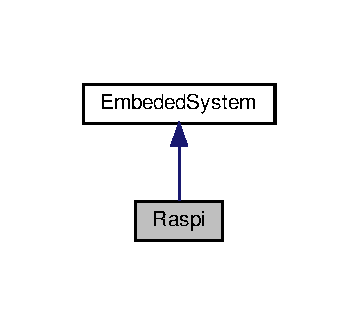
\includegraphics[width=172pt]{classRaspi__inherit__graph}
\end{center}
\end{figure}


Collaboration diagram for Raspi\+:\nopagebreak
\begin{figure}[H]
\begin{center}
\leavevmode
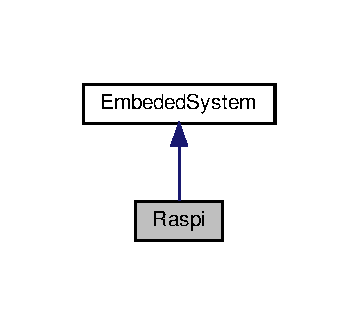
\includegraphics[width=172pt]{classRaspi__coll__graph}
\end{center}
\end{figure}
\subsection*{Public Member Functions}
\begin{DoxyCompactItemize}
\item 
void \hyperlink{classRaspi_adce86197732891370a63b239cc413c7e}{main} ()
\begin{DoxyCompactList}\small\item\em Funcion virtual pura que corre el main del SE. \end{DoxyCompactList}\end{DoxyCompactItemize}


\subsection{Detailed Description}
Clase que representa la Raspberry El metodo main es el bucle infinito del SE. 

Definition at line 73 of file robsim.\+h.



\subsection{Member Function Documentation}
\mbox{\Hypertarget{classRaspi_adce86197732891370a63b239cc413c7e}\label{classRaspi_adce86197732891370a63b239cc413c7e}} 
\index{Raspi@{Raspi}!main@{main}}
\index{main@{main}!Raspi@{Raspi}}
\subsubsection{\texorpdfstring{main()}{main()}}
{\footnotesize\ttfamily void Raspi\+::main (\begin{DoxyParamCaption}{ }\end{DoxyParamCaption})\hspace{0.3cm}{\ttfamily [virtual]}}



Funcion virtual pura que corre el main del SE. 



Implements \hyperlink{classEmbededSystem_a3a333d4954af4068f5e97301b4f55c48}{Embeded\+System}.



Definition at line 291 of file robsim.\+cpp.



The documentation for this class was generated from the following files\+:\begin{DoxyCompactItemize}
\item 
src/\hyperlink{robsim_8h}{robsim.\+h}\item 
src/\hyperlink{robsim_8cpp}{robsim.\+cpp}\end{DoxyCompactItemize}

\hypertarget{classSensor}{}\section{Sensor Class Reference}
\label{classSensor}\index{Sensor@{Sensor}}


Clase base sensores.  




{\ttfamily \#include $<$robsim.\+h$>$}



Inheritance diagram for Sensor\+:\nopagebreak
\begin{figure}[H]
\begin{center}
\leavevmode
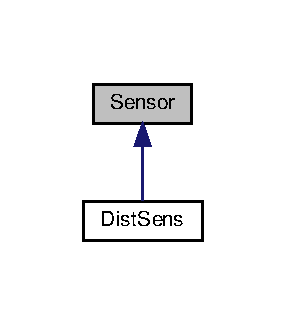
\includegraphics[width=137pt]{classSensor__inherit__graph}
\end{center}
\end{figure}


\subsection{Detailed Description}
Clase base sensores. 

Definition at line 127 of file robsim.\+h.



The documentation for this class was generated from the following file\+:\begin{DoxyCompactItemize}
\item 
src/\hyperlink{robsim_8h}{robsim.\+h}\end{DoxyCompactItemize}

\hypertarget{classTelemetryMsg}{}\section{Telemetry\+Msg Class Reference}
\label{classTelemetryMsg}\index{Telemetry\+Msg@{Telemetry\+Msg}}


Clase mensaje de telemetria.  




{\ttfamily \#include $<$robsim.\+h$>$}



Inheritance diagram for Telemetry\+Msg\+:\nopagebreak
\begin{figure}[H]
\begin{center}
\leavevmode
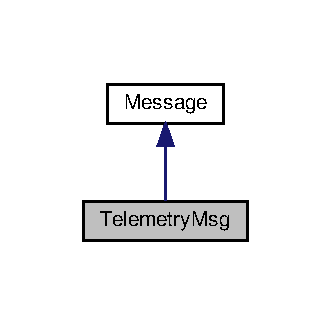
\includegraphics[width=159pt]{classTelemetryMsg__inherit__graph}
\end{center}
\end{figure}


Collaboration diagram for Telemetry\+Msg\+:\nopagebreak
\begin{figure}[H]
\begin{center}
\leavevmode
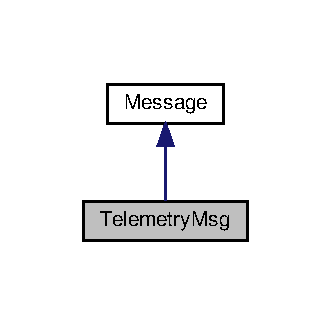
\includegraphics[width=159pt]{classTelemetryMsg__coll__graph}
\end{center}
\end{figure}
\subsection*{Public Member Functions}
\begin{DoxyCompactItemize}
\item 
\hyperlink{classTelemetryMsg_a930ff1a498097417aa25896e5ab92395}{Telemetry\+Msg} ()
\item 
void \hyperlink{classTelemetryMsg_a9c4b738c7a5fdbbaba534160de4f0ef1}{write\+\_\+\+I\+MU} (double I\+M\+Ux, double I\+M\+Uy, double I\+M\+Uz)
\begin{DoxyCompactList}\small\item\em Metodo que recibe los valores de aceleración de la I\+MU y lo escribe en un msj (atributo de clase base. \end{DoxyCompactList}\end{DoxyCompactItemize}
\subsection*{Additional Inherited Members}


\subsection{Detailed Description}
Clase mensaje de telemetria. 

Definition at line 159 of file robsim.\+h.



\subsection{Constructor \& Destructor Documentation}
\mbox{\Hypertarget{classTelemetryMsg_a930ff1a498097417aa25896e5ab92395}\label{classTelemetryMsg_a930ff1a498097417aa25896e5ab92395}} 
\index{Telemetry\+Msg@{Telemetry\+Msg}!Telemetry\+Msg@{Telemetry\+Msg}}
\index{Telemetry\+Msg@{Telemetry\+Msg}!Telemetry\+Msg@{Telemetry\+Msg}}
\subsubsection{\texorpdfstring{Telemetry\+Msg()}{TelemetryMsg()}}
{\footnotesize\ttfamily Telemetry\+Msg\+::\+Telemetry\+Msg (\begin{DoxyParamCaption}\item[{void}]{ }\end{DoxyParamCaption})}



Definition at line 104 of file robsim.\+cpp.



\subsection{Member Function Documentation}
\mbox{\Hypertarget{classTelemetryMsg_a9c4b738c7a5fdbbaba534160de4f0ef1}\label{classTelemetryMsg_a9c4b738c7a5fdbbaba534160de4f0ef1}} 
\index{Telemetry\+Msg@{Telemetry\+Msg}!write\+\_\+\+I\+MU@{write\+\_\+\+I\+MU}}
\index{write\+\_\+\+I\+MU@{write\+\_\+\+I\+MU}!Telemetry\+Msg@{Telemetry\+Msg}}
\subsubsection{\texorpdfstring{write\+\_\+\+I\+M\+U()}{write\_IMU()}}
{\footnotesize\ttfamily void Telemetry\+Msg\+::write\+\_\+\+I\+MU (\begin{DoxyParamCaption}\item[{double}]{I\+M\+Ux,  }\item[{double}]{I\+M\+Uy,  }\item[{double}]{I\+M\+Uz }\end{DoxyParamCaption})}



Metodo que recibe los valores de aceleración de la I\+MU y lo escribe en un msj (atributo de clase base. 


\begin{DoxyParams}[1]{Parameters}
\mbox{\tt in}  & {\em I\+M\+Ux} & Aceleración en x medida por la I\+MU \\
\hline
\mbox{\tt in}  & {\em I\+M\+Uy} & Aceleración en y medida por la I\+MU \\
\hline
\mbox{\tt in}  & {\em I\+M\+Uz} & Aceleración en z medida por la I\+MU \\
\hline
\end{DoxyParams}


Definition at line 127 of file robsim.\+cpp.



The documentation for this class was generated from the following files\+:\begin{DoxyCompactItemize}
\item 
src/\hyperlink{robsim_8h}{robsim.\+h}\item 
src/\hyperlink{robsim_8cpp}{robsim.\+cpp}\end{DoxyCompactItemize}

\hypertarget{classTimer}{}\section{Timer Class Reference}
\label{classTimer}\index{Timer@{Timer}}


Create asynchronous timers which execute specified functions in set time interval.  




{\ttfamily \#include $<$timer.\+h$>$}

\subsection*{Public Member Functions}
\begin{DoxyCompactItemize}
\item 
\hyperlink{classTimer_a5f16e8da27d2a5a5242dead46de05d97}{Timer} ()
\item 
\hyperlink{classTimer_a6e5fa1d67967d471f368218e1d0ae807}{Timer} (std\+::function$<$ void(void)$>$ func, const long \&interval)
\item 
void \hyperlink{classTimer_a3a8b5272198d029779dc9302a54305a8}{start} ()
\begin{DoxyCompactList}\small\item\em Starting the timer. \end{DoxyCompactList}\item 
void \hyperlink{classTimer_a63f0eb44b27402196590a03781515dba}{stop} ()
\item 
void \hyperlink{classTimer_aa3f7871196bb56202af2bc982bfbfff6}{restart} ()
\item 
bool \hyperlink{classTimer_a2ef50bfc604ea9fb88d3000c9ad0edd9}{is\+Running} ()
\item 
\hyperlink{classTimer}{Timer} $\ast$ \hyperlink{classTimer_a70653847aa7ae39d66379597e37db6af}{set\+Func} (std\+::function$<$ void(void)$>$ func)
\item 
long \hyperlink{classTimer_a0da8462797c35f5a91e7246eeed32198}{get\+Interval} ()
\item 
\hyperlink{classTimer}{Timer} $\ast$ \hyperlink{classTimer_abdc4f70c2dc58ee37b62861c842b77f0}{set\+Interval} (const long \&interval)
\item 
\hyperlink{classTimer_a14fa469c4c295c5fa6e66a4ad1092146}{$\sim$\+Timer} ()
\end{DoxyCompactItemize}


\subsection{Detailed Description}
Create asynchronous timers which execute specified functions in set time interval. 


\begin{DoxyParams}{Parameters}
{\em func} & Function which sould be executed \\
\hline
{\em interval} & Interval of time in which function will be executed (in milliseconds) \\
\hline
\end{DoxyParams}


Definition at line 22 of file timer.\+h.



\subsection{Constructor \& Destructor Documentation}
\mbox{\Hypertarget{classTimer_a5f16e8da27d2a5a5242dead46de05d97}\label{classTimer_a5f16e8da27d2a5a5242dead46de05d97}} 
\index{Timer@{Timer}!Timer@{Timer}}
\index{Timer@{Timer}!Timer@{Timer}}
\subsubsection{\texorpdfstring{Timer()}{Timer()}\hspace{0.1cm}{\footnotesize\ttfamily [1/2]}}
{\footnotesize\ttfamily Timer\+::\+Timer (\begin{DoxyParamCaption}{ }\end{DoxyParamCaption})\hspace{0.3cm}{\ttfamily [inline]}}



Definition at line 25 of file timer.\+h.

\mbox{\Hypertarget{classTimer_a6e5fa1d67967d471f368218e1d0ae807}\label{classTimer_a6e5fa1d67967d471f368218e1d0ae807}} 
\index{Timer@{Timer}!Timer@{Timer}}
\index{Timer@{Timer}!Timer@{Timer}}
\subsubsection{\texorpdfstring{Timer()}{Timer()}\hspace{0.1cm}{\footnotesize\ttfamily [2/2]}}
{\footnotesize\ttfamily Timer\+::\+Timer (\begin{DoxyParamCaption}\item[{std\+::function$<$ void(void)$>$}]{func,  }\item[{const long \&}]{interval }\end{DoxyParamCaption})\hspace{0.3cm}{\ttfamily [inline]}}



Definition at line 27 of file timer.\+h.

\mbox{\Hypertarget{classTimer_a14fa469c4c295c5fa6e66a4ad1092146}\label{classTimer_a14fa469c4c295c5fa6e66a4ad1092146}} 
\index{Timer@{Timer}!````~Timer@{$\sim$\+Timer}}
\index{````~Timer@{$\sim$\+Timer}!Timer@{Timer}}
\subsubsection{\texorpdfstring{$\sim$\+Timer()}{~Timer()}}
{\footnotesize\ttfamily Timer\+::$\sim$\+Timer (\begin{DoxyParamCaption}{ }\end{DoxyParamCaption})\hspace{0.3cm}{\ttfamily [inline]}}



Definition at line 108 of file timer.\+h.



\subsection{Member Function Documentation}
\mbox{\Hypertarget{classTimer_a0da8462797c35f5a91e7246eeed32198}\label{classTimer_a0da8462797c35f5a91e7246eeed32198}} 
\index{Timer@{Timer}!get\+Interval@{get\+Interval}}
\index{get\+Interval@{get\+Interval}!Timer@{Timer}}
\subsubsection{\texorpdfstring{get\+Interval()}{getInterval()}}
{\footnotesize\ttfamily long Timer\+::get\+Interval (\begin{DoxyParamCaption}{ }\end{DoxyParamCaption})\hspace{0.3cm}{\ttfamily [inline]}}



Definition at line 91 of file timer.\+h.

\mbox{\Hypertarget{classTimer_a2ef50bfc604ea9fb88d3000c9ad0edd9}\label{classTimer_a2ef50bfc604ea9fb88d3000c9ad0edd9}} 
\index{Timer@{Timer}!is\+Running@{is\+Running}}
\index{is\+Running@{is\+Running}!Timer@{Timer}}
\subsubsection{\texorpdfstring{is\+Running()}{isRunning()}}
{\footnotesize\ttfamily bool Timer\+::is\+Running (\begin{DoxyParamCaption}{ }\end{DoxyParamCaption})\hspace{0.3cm}{\ttfamily [inline]}}



Definition at line 69 of file timer.\+h.

\mbox{\Hypertarget{classTimer_aa3f7871196bb56202af2bc982bfbfff6}\label{classTimer_aa3f7871196bb56202af2bc982bfbfff6}} 
\index{Timer@{Timer}!restart@{restart}}
\index{restart@{restart}!Timer@{Timer}}
\subsubsection{\texorpdfstring{restart()}{restart()}}
{\footnotesize\ttfamily void Timer\+::restart (\begin{DoxyParamCaption}{ }\end{DoxyParamCaption})\hspace{0.3cm}{\ttfamily [inline]}}



Definition at line 59 of file timer.\+h.

\mbox{\Hypertarget{classTimer_a70653847aa7ae39d66379597e37db6af}\label{classTimer_a70653847aa7ae39d66379597e37db6af}} 
\index{Timer@{Timer}!set\+Func@{set\+Func}}
\index{set\+Func@{set\+Func}!Timer@{Timer}}
\subsubsection{\texorpdfstring{set\+Func()}{setFunc()}}
{\footnotesize\ttfamily \hyperlink{classTimer}{Timer}$\ast$ Timer\+::set\+Func (\begin{DoxyParamCaption}\item[{std\+::function$<$ void(void)$>$}]{func }\end{DoxyParamCaption})\hspace{0.3cm}{\ttfamily [inline]}}



Definition at line 81 of file timer.\+h.

\mbox{\Hypertarget{classTimer_abdc4f70c2dc58ee37b62861c842b77f0}\label{classTimer_abdc4f70c2dc58ee37b62861c842b77f0}} 
\index{Timer@{Timer}!set\+Interval@{set\+Interval}}
\index{set\+Interval@{set\+Interval}!Timer@{Timer}}
\subsubsection{\texorpdfstring{set\+Interval()}{setInterval()}}
{\footnotesize\ttfamily \hyperlink{classTimer}{Timer}$\ast$ Timer\+::set\+Interval (\begin{DoxyParamCaption}\item[{const long \&}]{interval }\end{DoxyParamCaption})\hspace{0.3cm}{\ttfamily [inline]}}



Definition at line 103 of file timer.\+h.

\mbox{\Hypertarget{classTimer_a3a8b5272198d029779dc9302a54305a8}\label{classTimer_a3a8b5272198d029779dc9302a54305a8}} 
\index{Timer@{Timer}!start@{start}}
\index{start@{start}!Timer@{Timer}}
\subsubsection{\texorpdfstring{start()}{start()}}
{\footnotesize\ttfamily void Timer\+::start (\begin{DoxyParamCaption}{ }\end{DoxyParamCaption})\hspace{0.3cm}{\ttfamily [inline]}}



Starting the timer. 



Definition at line 35 of file timer.\+h.

\mbox{\Hypertarget{classTimer_a63f0eb44b27402196590a03781515dba}\label{classTimer_a63f0eb44b27402196590a03781515dba}} 
\index{Timer@{Timer}!stop@{stop}}
\index{stop@{stop}!Timer@{Timer}}
\subsubsection{\texorpdfstring{stop()}{stop()}}
{\footnotesize\ttfamily void Timer\+::stop (\begin{DoxyParamCaption}{ }\end{DoxyParamCaption})\hspace{0.3cm}{\ttfamily [inline]}}



Definition at line 50 of file timer.\+h.



The documentation for this class was generated from the following file\+:\begin{DoxyCompactItemize}
\item 
src/\hyperlink{timer_8h}{timer.\+h}\end{DoxyCompactItemize}

\chapter{File Documentation}
\hypertarget{main_8cpp}{}\section{main.\+cpp File Reference}
\label{main_8cpp}\index{main.\+cpp@{main.\+cpp}}
{\ttfamily \#include $<$iostream$>$}\newline
Include dependency graph for main.\+cpp\+:\nopagebreak
\begin{figure}[H]
\begin{center}
\leavevmode
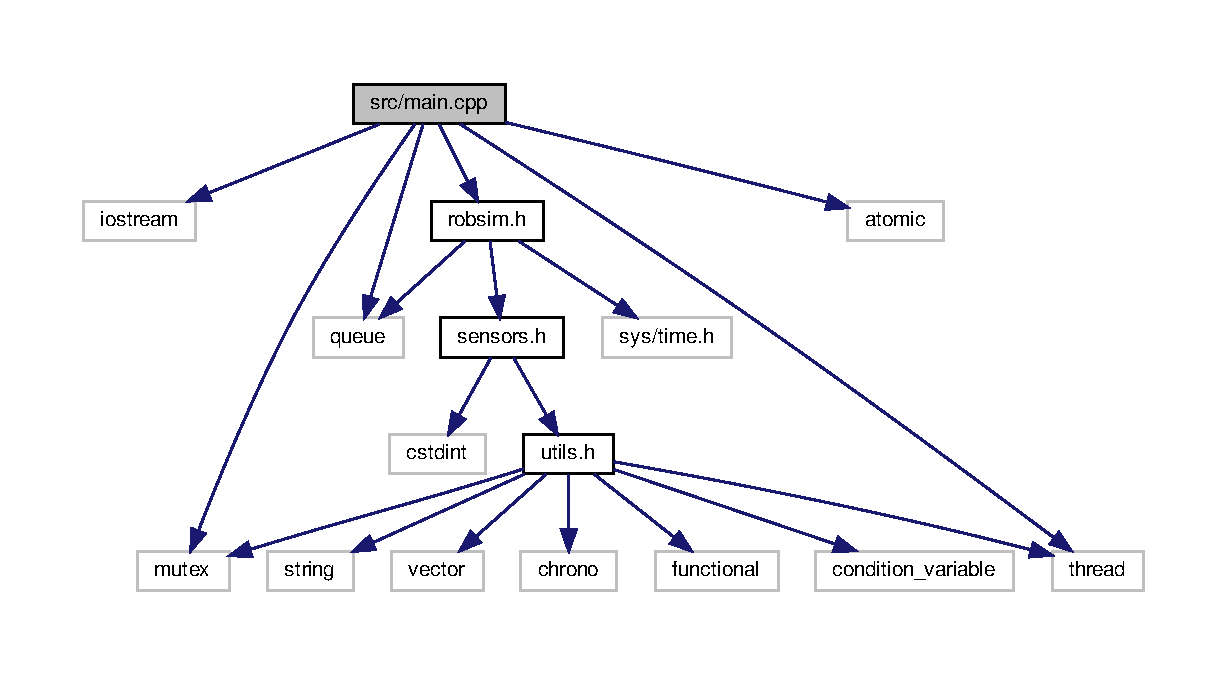
\includegraphics[width=136pt]{main_8cpp__incl}
\end{center}
\end{figure}
\subsection*{Functions}
\begin{DoxyCompactItemize}
\item 
\mbox{\Hypertarget{main_8cpp_ae66f6b31b5ad750f1fe042a706a4e3d4}\label{main_8cpp_ae66f6b31b5ad750f1fe042a706a4e3d4}} 
int {\bfseries main} ()
\end{DoxyCompactItemize}

\hypertarget{main_8md}{}\section{src/main.md File Reference}
\label{main_8md}\index{src/main.\+md@{src/main.\+md}}

\hypertarget{Readme_8md}{}\section{src/\+Readme.md File Reference}
\label{Readme_8md}\index{src/\+Readme.\+md@{src/\+Readme.\+md}}

\hypertarget{robsim_8cpp}{}\section{src/robsim.cpp File Reference}
\label{robsim_8cpp}\index{src/robsim.\+cpp@{src/robsim.\+cpp}}
{\ttfamily \#include $<$iostream$>$}\newline
{\ttfamily \#include $<$queue$>$}\newline
{\ttfamily \#include $<$mutex$>$}\newline
{\ttfamily \#include $<$thread$>$}\newline
{\ttfamily \#include $<$vector$>$}\newline
{\ttfamily \#include $<$iomanip$>$}\newline
{\ttfamily \#include $<$atomic$>$}\newline
{\ttfamily \#include $<$cmath$>$}\newline
{\ttfamily \#include \char`\"{}sensors.\+h\char`\"{}}\newline
{\ttfamily \#include \char`\"{}robsim.\+h\char`\"{}}\newline
{\ttfamily \#include \char`\"{}utils.\+h\char`\"{}}\newline
{\ttfamily \#include \char`\"{}timer.\+h\char`\"{}}\newline
Include dependency graph for robsim.\+cpp\+:\nopagebreak
\begin{figure}[H]
\begin{center}
\leavevmode
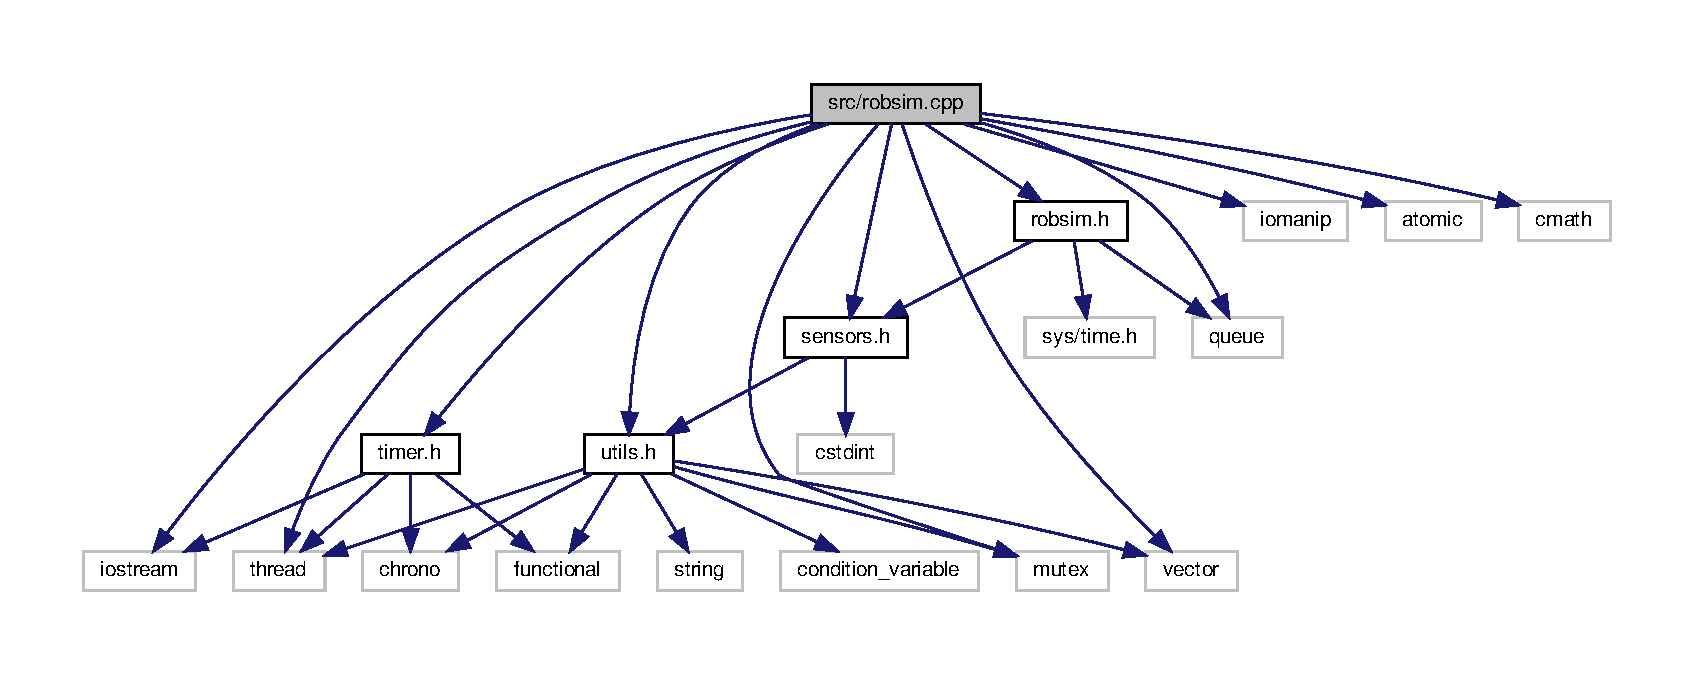
\includegraphics[width=350pt]{robsim_8cpp__incl}
\end{center}
\end{figure}
\subsection*{Macros}
\begin{DoxyCompactItemize}
\item 
\#define \hyperlink{robsim_8cpp_a7ac2ec469c5986de6309d55a49dece55}{S\+A\+M\+P\+L\+E\+\_\+\+T\+I\+M\+E\+\_\+\+A\+R\+D\+U\+I\+NO}~0.\+1;
\item 
\#define \hyperlink{robsim_8cpp_a19199de75b4f4eb26cb503afea095e91}{S\+A\+M\+P\+L\+E\+\_\+\+T\+I\+M\+E\+\_\+\+C\+A\+M\+E\+RA}~0.\+1;
\item 
\#define \hyperlink{robsim_8cpp_acc46c880b139b5895f6a8236b3aff526}{S\+A\+M\+P\+L\+E\+\_\+\+T\+I\+M\+E\+\_\+\+R\+A\+S\+PI}~0.\+1;
\end{DoxyCompactItemize}
\subsection*{Functions}
\begin{DoxyCompactItemize}
\item 
int \hyperlink{robsim_8cpp_abfd055405fc0db9a96a29057436d7e6b}{time\+\_\+falt\+\_\+next\+\_\+interv\+\_\+ms} (struct timeval $\ast$t0, int n, double dt)
\begin{DoxyCompactList}\small\item\em Calcula el tiempo faltante para el siguiente intervalo. \end{DoxyCompactList}\item 
void \hyperlink{robsim_8cpp_ae9bdf1cf8a02cfad30e904f75ede4f4e}{espera\+\_\+siguiente\+\_\+intervalo} (struct timeval $\ast$t0, int n, double dt)
\begin{DoxyCompactList}\small\item\em Función bloqueante que espera hasta el siguiente intervalor. \end{DoxyCompactList}\item 
void \hyperlink{robsim_8cpp_a40a893993ca0fba530429f44aa0b176f}{f} (bool $\ast$flag)
\item 
void \hyperlink{robsim_8cpp_a075142c6dceedf39581a5038d5c9edf7}{Cam\+Th} ()
\end{DoxyCompactItemize}


\subsection{Macro Definition Documentation}
\mbox{\Hypertarget{robsim_8cpp_a7ac2ec469c5986de6309d55a49dece55}\label{robsim_8cpp_a7ac2ec469c5986de6309d55a49dece55}} 
\index{robsim.\+cpp@{robsim.\+cpp}!S\+A\+M\+P\+L\+E\+\_\+\+T\+I\+M\+E\+\_\+\+A\+R\+D\+U\+I\+NO@{S\+A\+M\+P\+L\+E\+\_\+\+T\+I\+M\+E\+\_\+\+A\+R\+D\+U\+I\+NO}}
\index{S\+A\+M\+P\+L\+E\+\_\+\+T\+I\+M\+E\+\_\+\+A\+R\+D\+U\+I\+NO@{S\+A\+M\+P\+L\+E\+\_\+\+T\+I\+M\+E\+\_\+\+A\+R\+D\+U\+I\+NO}!robsim.\+cpp@{robsim.\+cpp}}
\subsubsection{\texorpdfstring{S\+A\+M\+P\+L\+E\+\_\+\+T\+I\+M\+E\+\_\+\+A\+R\+D\+U\+I\+NO}{SAMPLE\_TIME\_ARDUINO}}
{\footnotesize\ttfamily \#define S\+A\+M\+P\+L\+E\+\_\+\+T\+I\+M\+E\+\_\+\+A\+R\+D\+U\+I\+NO~0.\+1;}



Definition at line 18 of file robsim.\+cpp.

\mbox{\Hypertarget{robsim_8cpp_a19199de75b4f4eb26cb503afea095e91}\label{robsim_8cpp_a19199de75b4f4eb26cb503afea095e91}} 
\index{robsim.\+cpp@{robsim.\+cpp}!S\+A\+M\+P\+L\+E\+\_\+\+T\+I\+M\+E\+\_\+\+C\+A\+M\+E\+RA@{S\+A\+M\+P\+L\+E\+\_\+\+T\+I\+M\+E\+\_\+\+C\+A\+M\+E\+RA}}
\index{S\+A\+M\+P\+L\+E\+\_\+\+T\+I\+M\+E\+\_\+\+C\+A\+M\+E\+RA@{S\+A\+M\+P\+L\+E\+\_\+\+T\+I\+M\+E\+\_\+\+C\+A\+M\+E\+RA}!robsim.\+cpp@{robsim.\+cpp}}
\subsubsection{\texorpdfstring{S\+A\+M\+P\+L\+E\+\_\+\+T\+I\+M\+E\+\_\+\+C\+A\+M\+E\+RA}{SAMPLE\_TIME\_CAMERA}}
{\footnotesize\ttfamily \#define S\+A\+M\+P\+L\+E\+\_\+\+T\+I\+M\+E\+\_\+\+C\+A\+M\+E\+RA~0.\+1;}



Definition at line 19 of file robsim.\+cpp.

\mbox{\Hypertarget{robsim_8cpp_acc46c880b139b5895f6a8236b3aff526}\label{robsim_8cpp_acc46c880b139b5895f6a8236b3aff526}} 
\index{robsim.\+cpp@{robsim.\+cpp}!S\+A\+M\+P\+L\+E\+\_\+\+T\+I\+M\+E\+\_\+\+R\+A\+S\+PI@{S\+A\+M\+P\+L\+E\+\_\+\+T\+I\+M\+E\+\_\+\+R\+A\+S\+PI}}
\index{S\+A\+M\+P\+L\+E\+\_\+\+T\+I\+M\+E\+\_\+\+R\+A\+S\+PI@{S\+A\+M\+P\+L\+E\+\_\+\+T\+I\+M\+E\+\_\+\+R\+A\+S\+PI}!robsim.\+cpp@{robsim.\+cpp}}
\subsubsection{\texorpdfstring{S\+A\+M\+P\+L\+E\+\_\+\+T\+I\+M\+E\+\_\+\+R\+A\+S\+PI}{SAMPLE\_TIME\_RASPI}}
{\footnotesize\ttfamily \#define S\+A\+M\+P\+L\+E\+\_\+\+T\+I\+M\+E\+\_\+\+R\+A\+S\+PI~0.\+1;}



Definition at line 20 of file robsim.\+cpp.



\subsection{Function Documentation}
\mbox{\Hypertarget{robsim_8cpp_a075142c6dceedf39581a5038d5c9edf7}\label{robsim_8cpp_a075142c6dceedf39581a5038d5c9edf7}} 
\index{robsim.\+cpp@{robsim.\+cpp}!Cam\+Th@{Cam\+Th}}
\index{Cam\+Th@{Cam\+Th}!robsim.\+cpp@{robsim.\+cpp}}
\subsubsection{\texorpdfstring{Cam\+Th()}{CamTh()}}
{\footnotesize\ttfamily void Cam\+Th (\begin{DoxyParamCaption}{ }\end{DoxyParamCaption})}



Definition at line 286 of file robsim.\+cpp.

\mbox{\Hypertarget{robsim_8cpp_ae9bdf1cf8a02cfad30e904f75ede4f4e}\label{robsim_8cpp_ae9bdf1cf8a02cfad30e904f75ede4f4e}} 
\index{robsim.\+cpp@{robsim.\+cpp}!espera\+\_\+siguiente\+\_\+intervalo@{espera\+\_\+siguiente\+\_\+intervalo}}
\index{espera\+\_\+siguiente\+\_\+intervalo@{espera\+\_\+siguiente\+\_\+intervalo}!robsim.\+cpp@{robsim.\+cpp}}
\subsubsection{\texorpdfstring{espera\+\_\+siguiente\+\_\+intervalo()}{espera\_siguiente\_intervalo()}}
{\footnotesize\ttfamily void espera\+\_\+siguiente\+\_\+intervalo (\begin{DoxyParamCaption}\item[{struct timeval $\ast$}]{t0,  }\item[{int}]{n,  }\item[{double}]{dt }\end{DoxyParamCaption})}



Función bloqueante que espera hasta el siguiente intervalor. 


\begin{DoxyParams}[1]{Parameters}
\mbox{\tt in}  & {\em $\ast$t0} & puntero a timeval con el tiempo incial del experimento \\
\hline
\mbox{\tt in}  & {\em n} & numero de intervalo \\
\hline
\mbox{\tt in}  & {\em dt} & paso de tiempo \\
\hline
\end{DoxyParams}


Definition at line 34 of file robsim.\+cpp.

\mbox{\Hypertarget{robsim_8cpp_a40a893993ca0fba530429f44aa0b176f}\label{robsim_8cpp_a40a893993ca0fba530429f44aa0b176f}} 
\index{robsim.\+cpp@{robsim.\+cpp}!f@{f}}
\index{f@{f}!robsim.\+cpp@{robsim.\+cpp}}
\subsubsection{\texorpdfstring{f()}{f()}}
{\footnotesize\ttfamily void f (\begin{DoxyParamCaption}\item[{bool $\ast$}]{flag }\end{DoxyParamCaption})}



Definition at line 209 of file robsim.\+cpp.

\mbox{\Hypertarget{robsim_8cpp_abfd055405fc0db9a96a29057436d7e6b}\label{robsim_8cpp_abfd055405fc0db9a96a29057436d7e6b}} 
\index{robsim.\+cpp@{robsim.\+cpp}!time\+\_\+falt\+\_\+next\+\_\+interv\+\_\+ms@{time\+\_\+falt\+\_\+next\+\_\+interv\+\_\+ms}}
\index{time\+\_\+falt\+\_\+next\+\_\+interv\+\_\+ms@{time\+\_\+falt\+\_\+next\+\_\+interv\+\_\+ms}!robsim.\+cpp@{robsim.\+cpp}}
\subsubsection{\texorpdfstring{time\+\_\+falt\+\_\+next\+\_\+interv\+\_\+ms()}{time\_falt\_next\_interv\_ms()}}
{\footnotesize\ttfamily int time\+\_\+falt\+\_\+next\+\_\+interv\+\_\+ms (\begin{DoxyParamCaption}\item[{struct timeval $\ast$}]{t0,  }\item[{int}]{n,  }\item[{double}]{dt }\end{DoxyParamCaption})}



Calcula el tiempo faltante para el siguiente intervalo. 


\begin{DoxyParams}[1]{Parameters}
\mbox{\tt in}  & {\em $\ast$t0} & puntero a timeval con el tiempo incial del experimento \\
\hline
\mbox{\tt in}  & {\em n} & numero de intervalor \\
\hline
\mbox{\tt in}  & {\em dt} & paso de tiempo\\
\hline
\end{DoxyParams}
\begin{DoxyReturn}{Returns}
Tiempo en ms hasta el intervalo n 
\end{DoxyReturn}


Definition at line 25 of file robsim.\+cpp.


\hypertarget{robsim_8h}{}\section{src/robsim.h File Reference}
\label{robsim_8h}\index{src/robsim.\+h@{src/robsim.\+h}}
{\ttfamily \#include $<$queue$>$}\newline
{\ttfamily \#include \char`\"{}sensors.\+h\char`\"{}}\newline
{\ttfamily \#include $<$sys/time.\+h$>$}\newline
Include dependency graph for robsim.\+h\+:\nopagebreak
\begin{figure}[H]
\begin{center}
\leavevmode
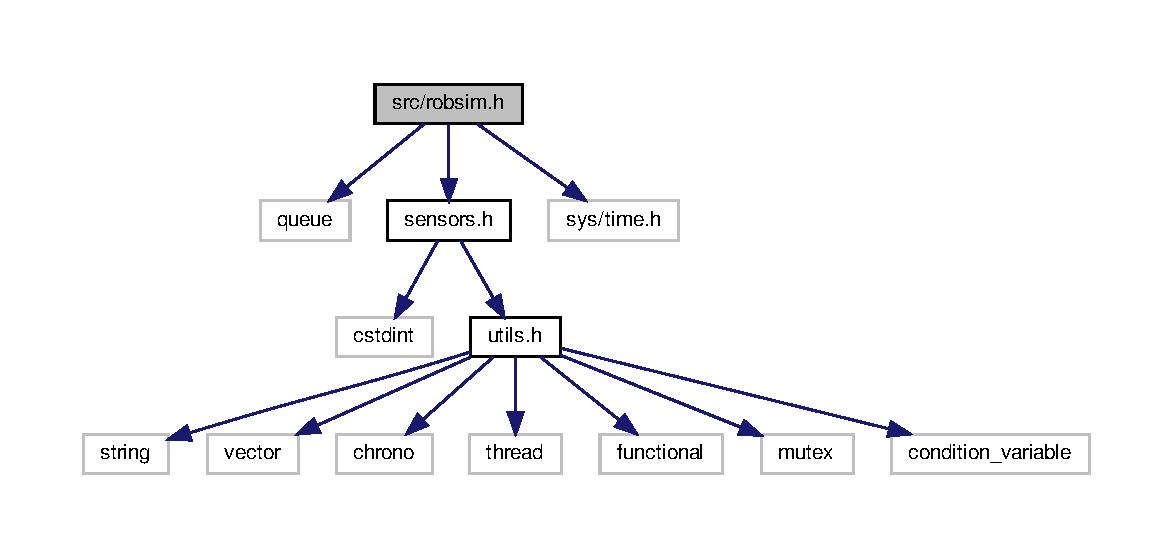
\includegraphics[width=350pt]{robsim_8h__incl}
\end{center}
\end{figure}
This graph shows which files directly or indirectly include this file\+:\nopagebreak
\begin{figure}[H]
\begin{center}
\leavevmode
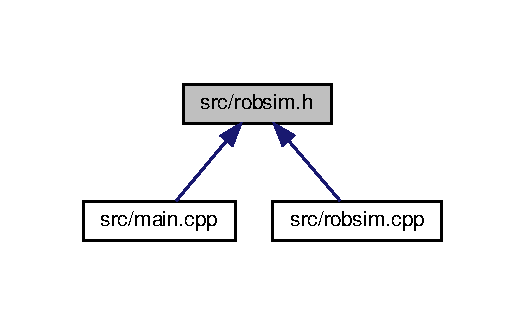
\includegraphics[width=252pt]{robsim_8h__dep__incl}
\end{center}
\end{figure}
\subsection*{Classes}
\begin{DoxyCompactItemize}
\item 
class \hyperlink{classEmbededSystem}{Embeded\+System}
\begin{DoxyCompactList}\small\item\em a Clase base Sistema embebido Tiene como metodo virtual puro el main de los SE \end{DoxyCompactList}\item 
class \hyperlink{classArduinoR}{ArduinoR}
\begin{DoxyCompactList}\small\item\em Clase que representa el Arduino dedicado al sistema 1 El metodo main es el bucle infinito del SE Hereda de la clase Sistema Embebido. \end{DoxyCompactList}\item 
class \hyperlink{classArduinoL}{ArduinoL}
\begin{DoxyCompactList}\small\item\em Clase que representa el Arduino dedicado al sistema 2 El metodo main es el bucle infinito del SE. \end{DoxyCompactList}\item 
class \hyperlink{classRaspi}{Raspi}
\begin{DoxyCompactList}\small\item\em Clase que representa la Raspberry El metodo main es el bucle infinito del SE. \end{DoxyCompactList}\item 
class \hyperlink{classCamera}{Camera}
\begin{DoxyCompactList}\small\item\em Clase que representa la camara El metodo main es el bucle infinito del SE. \end{DoxyCompactList}\item 
class \hyperlink{classActuator}{Actuator}
\begin{DoxyCompactList}\small\item\em Clase base actuadores. \end{DoxyCompactList}\item 
class \hyperlink{classJetPump}{Jet\+Pump}
\begin{DoxyCompactList}\small\item\em Clase \hyperlink{classJetPump}{Jet\+Pump}. \end{DoxyCompactList}\item 
class \hyperlink{classSensor}{Sensor}
\begin{DoxyCompactList}\small\item\em Clase base sensores. \end{DoxyCompactList}\item 
class \hyperlink{classDistSens}{Dist\+Sens}
\begin{DoxyCompactList}\small\item\em Clase que representa el sensor de dist. \end{DoxyCompactList}\item 
class \hyperlink{classMessage}{Message}
\begin{DoxyCompactList}\small\item\em Clase Mensaje. \end{DoxyCompactList}\item 
class \hyperlink{classTelemetryMsg}{Telemetry\+Msg}
\begin{DoxyCompactList}\small\item\em Clase mensaje de telemetria. \end{DoxyCompactList}\item 
class \hyperlink{classActionMsg}{Action\+Msg}
\begin{DoxyCompactList}\small\item\em Clase mensaje de accion de control. \end{DoxyCompactList}\item 
class \hyperlink{classCameraMsg}{Camera\+Msg}
\begin{DoxyCompactList}\small\item\em Clase mensaje de camara. \end{DoxyCompactList}\end{DoxyCompactItemize}
\subsection*{Macros}
\begin{DoxyCompactItemize}
\item 
\#define \hyperlink{robsim_8h_a6a7d0aa2f8672b5fd4207bf9a4d2912d}{M\+S\+G\+\_\+\+T\+E\+L\+E\+M\+E\+T\+RY}~\hyperlink{classMessage_a1c65ab3f02ba5b175f583f9d275ecf2babb3d2d909c73fe49800949a344775f8b}{Message\+::\+Type\+::\+T\+E\+L\+E\+M\+E\+T\+RY}
\item 
\#define \hyperlink{robsim_8h_add686b3cb16e812ad19e05944997c2a7}{M\+S\+G\+\_\+\+A\+C\+T\+I\+ON}~\hyperlink{classMessage_a1c65ab3f02ba5b175f583f9d275ecf2bae58a1b00942e66d8b4abc960da7877ab}{Message\+::\+Type\+::\+A\+C\+T\+I\+ON}
\item 
\#define \hyperlink{robsim_8h_ad066d2f092a3d1bb49aca1f9524c66c3}{M\+S\+G\+\_\+\+C\+A\+M\+E\+RA}~\hyperlink{classMessage_a1c65ab3f02ba5b175f583f9d275ecf2baddf0d6b21537d984fea6544f58101fa8}{Message\+::\+Type\+::\+C\+A\+M\+E\+RA}
\end{DoxyCompactItemize}
\subsection*{Functions}
\begin{DoxyCompactItemize}
\item 
int \hyperlink{robsim_8h_abfd055405fc0db9a96a29057436d7e6b}{time\+\_\+falt\+\_\+next\+\_\+interv\+\_\+ms} (struct timeval $\ast$t0, int n, double dt)
\begin{DoxyCompactList}\small\item\em Calcula el tiempo faltante para el siguiente intervalo. \end{DoxyCompactList}\item 
void \hyperlink{robsim_8h_ae9bdf1cf8a02cfad30e904f75ede4f4e}{espera\+\_\+siguiente\+\_\+intervalo} (struct timeval $\ast$t0, int n, double dt)
\begin{DoxyCompactList}\small\item\em Función bloqueante que espera hasta el siguiente intervalor. \end{DoxyCompactList}\end{DoxyCompactItemize}


\subsection{Detailed Description}
\begin{DoxyAuthor}{Author}
Francisco Ortiz 
\end{DoxyAuthor}


\subsection{Macro Definition Documentation}
\mbox{\Hypertarget{robsim_8h_add686b3cb16e812ad19e05944997c2a7}\label{robsim_8h_add686b3cb16e812ad19e05944997c2a7}} 
\index{robsim.\+h@{robsim.\+h}!M\+S\+G\+\_\+\+A\+C\+T\+I\+ON@{M\+S\+G\+\_\+\+A\+C\+T\+I\+ON}}
\index{M\+S\+G\+\_\+\+A\+C\+T\+I\+ON@{M\+S\+G\+\_\+\+A\+C\+T\+I\+ON}!robsim.\+h@{robsim.\+h}}
\subsubsection{\texorpdfstring{M\+S\+G\+\_\+\+A\+C\+T\+I\+ON}{MSG\_ACTION}}
{\footnotesize\ttfamily \#define M\+S\+G\+\_\+\+A\+C\+T\+I\+ON~\hyperlink{classMessage_a1c65ab3f02ba5b175f583f9d275ecf2bae58a1b00942e66d8b4abc960da7877ab}{Message\+::\+Type\+::\+A\+C\+T\+I\+ON}}



Definition at line 15 of file robsim.\+h.

\mbox{\Hypertarget{robsim_8h_ad066d2f092a3d1bb49aca1f9524c66c3}\label{robsim_8h_ad066d2f092a3d1bb49aca1f9524c66c3}} 
\index{robsim.\+h@{robsim.\+h}!M\+S\+G\+\_\+\+C\+A\+M\+E\+RA@{M\+S\+G\+\_\+\+C\+A\+M\+E\+RA}}
\index{M\+S\+G\+\_\+\+C\+A\+M\+E\+RA@{M\+S\+G\+\_\+\+C\+A\+M\+E\+RA}!robsim.\+h@{robsim.\+h}}
\subsubsection{\texorpdfstring{M\+S\+G\+\_\+\+C\+A\+M\+E\+RA}{MSG\_CAMERA}}
{\footnotesize\ttfamily \#define M\+S\+G\+\_\+\+C\+A\+M\+E\+RA~\hyperlink{classMessage_a1c65ab3f02ba5b175f583f9d275ecf2baddf0d6b21537d984fea6544f58101fa8}{Message\+::\+Type\+::\+C\+A\+M\+E\+RA}}



Definition at line 16 of file robsim.\+h.

\mbox{\Hypertarget{robsim_8h_a6a7d0aa2f8672b5fd4207bf9a4d2912d}\label{robsim_8h_a6a7d0aa2f8672b5fd4207bf9a4d2912d}} 
\index{robsim.\+h@{robsim.\+h}!M\+S\+G\+\_\+\+T\+E\+L\+E\+M\+E\+T\+RY@{M\+S\+G\+\_\+\+T\+E\+L\+E\+M\+E\+T\+RY}}
\index{M\+S\+G\+\_\+\+T\+E\+L\+E\+M\+E\+T\+RY@{M\+S\+G\+\_\+\+T\+E\+L\+E\+M\+E\+T\+RY}!robsim.\+h@{robsim.\+h}}
\subsubsection{\texorpdfstring{M\+S\+G\+\_\+\+T\+E\+L\+E\+M\+E\+T\+RY}{MSG\_TELEMETRY}}
{\footnotesize\ttfamily \#define M\+S\+G\+\_\+\+T\+E\+L\+E\+M\+E\+T\+RY~\hyperlink{classMessage_a1c65ab3f02ba5b175f583f9d275ecf2babb3d2d909c73fe49800949a344775f8b}{Message\+::\+Type\+::\+T\+E\+L\+E\+M\+E\+T\+RY}}



Definition at line 14 of file robsim.\+h.



\subsection{Function Documentation}
\mbox{\Hypertarget{robsim_8h_ae9bdf1cf8a02cfad30e904f75ede4f4e}\label{robsim_8h_ae9bdf1cf8a02cfad30e904f75ede4f4e}} 
\index{robsim.\+h@{robsim.\+h}!espera\+\_\+siguiente\+\_\+intervalo@{espera\+\_\+siguiente\+\_\+intervalo}}
\index{espera\+\_\+siguiente\+\_\+intervalo@{espera\+\_\+siguiente\+\_\+intervalo}!robsim.\+h@{robsim.\+h}}
\subsubsection{\texorpdfstring{espera\+\_\+siguiente\+\_\+intervalo()}{espera\_siguiente\_intervalo()}}
{\footnotesize\ttfamily void espera\+\_\+siguiente\+\_\+intervalo (\begin{DoxyParamCaption}\item[{struct timeval $\ast$}]{t0,  }\item[{int}]{n,  }\item[{double}]{dt }\end{DoxyParamCaption})}



Función bloqueante que espera hasta el siguiente intervalor. 


\begin{DoxyParams}[1]{Parameters}
\mbox{\tt in}  & {\em $\ast$t0} & puntero a timeval con el tiempo incial del experimento \\
\hline
\mbox{\tt in}  & {\em n} & numero de intervalo \\
\hline
\mbox{\tt in}  & {\em dt} & paso de tiempo \\
\hline
\end{DoxyParams}


Definition at line 34 of file robsim.\+cpp.

\mbox{\Hypertarget{robsim_8h_abfd055405fc0db9a96a29057436d7e6b}\label{robsim_8h_abfd055405fc0db9a96a29057436d7e6b}} 
\index{robsim.\+h@{robsim.\+h}!time\+\_\+falt\+\_\+next\+\_\+interv\+\_\+ms@{time\+\_\+falt\+\_\+next\+\_\+interv\+\_\+ms}}
\index{time\+\_\+falt\+\_\+next\+\_\+interv\+\_\+ms@{time\+\_\+falt\+\_\+next\+\_\+interv\+\_\+ms}!robsim.\+h@{robsim.\+h}}
\subsubsection{\texorpdfstring{time\+\_\+falt\+\_\+next\+\_\+interv\+\_\+ms()}{time\_falt\_next\_interv\_ms()}}
{\footnotesize\ttfamily int time\+\_\+falt\+\_\+next\+\_\+interv\+\_\+ms (\begin{DoxyParamCaption}\item[{struct timeval $\ast$}]{t0,  }\item[{int}]{n,  }\item[{double}]{dt }\end{DoxyParamCaption})}



Calcula el tiempo faltante para el siguiente intervalo. 


\begin{DoxyParams}[1]{Parameters}
\mbox{\tt in}  & {\em $\ast$t0} & puntero a timeval con el tiempo incial del experimento \\
\hline
\mbox{\tt in}  & {\em n} & numero de intervalor \\
\hline
\mbox{\tt in}  & {\em dt} & paso de tiempo\\
\hline
\end{DoxyParams}
\begin{DoxyReturn}{Returns}
Tiempo en ms hasta el intervalo n 
\end{DoxyReturn}


Definition at line 25 of file robsim.\+cpp.


\hypertarget{sensors_8cpp}{}\section{src/sensors.cpp File Reference}
\label{sensors_8cpp}\index{src/sensors.\+cpp@{src/sensors.\+cpp}}
{\ttfamily \#include \char`\"{}sensors.\+h\char`\"{}}\newline
{\ttfamily \#include $<$iostream$>$}\newline
{\ttfamily \#include $<$cstdlib$>$}\newline
{\ttfamily \#include $<$ctime$>$}\newline
Include dependency graph for sensors.\+cpp\+:\nopagebreak
\begin{figure}[H]
\begin{center}
\leavevmode
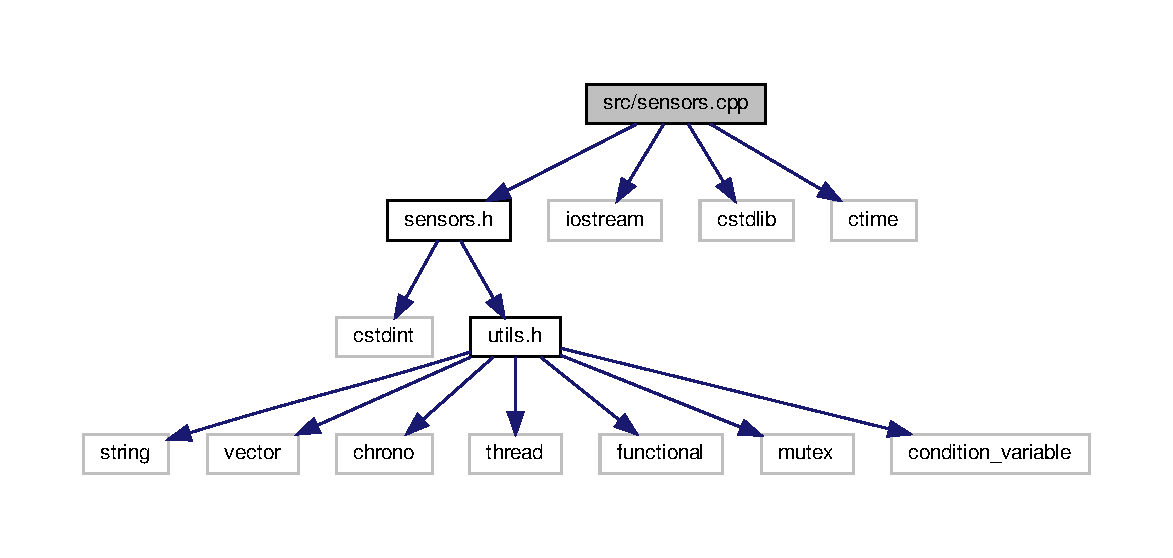
\includegraphics[width=350pt]{sensors_8cpp__incl}
\end{center}
\end{figure}

\hypertarget{sensors_8h}{}\section{src/sensors.h File Reference}
\label{sensors_8h}\index{src/sensors.\+h@{src/sensors.\+h}}
{\ttfamily \#include $<$cstdint$>$}\newline
{\ttfamily \#include \char`\"{}utils.\+h\char`\"{}}\newline
Include dependency graph for sensors.\+h\+:\nopagebreak
\begin{figure}[H]
\begin{center}
\leavevmode
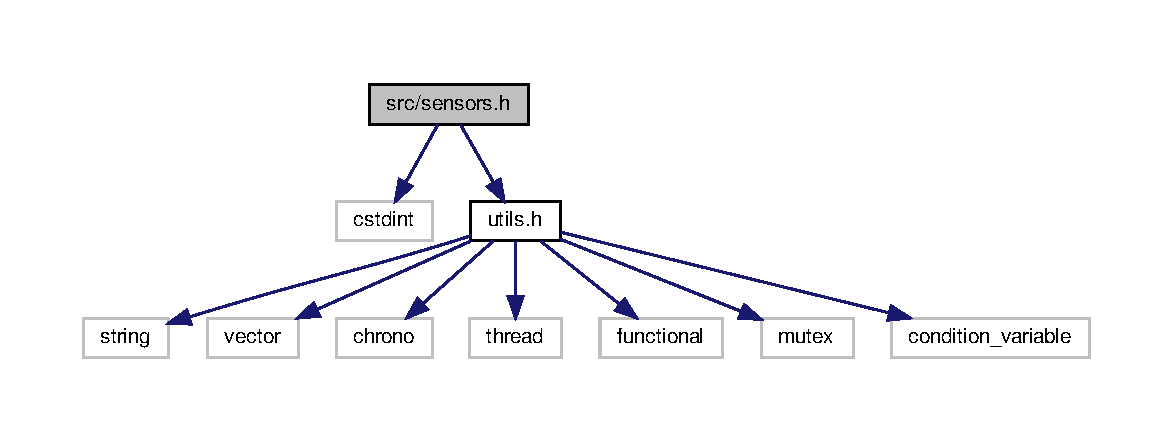
\includegraphics[width=350pt]{sensors_8h__incl}
\end{center}
\end{figure}
This graph shows which files directly or indirectly include this file\+:\nopagebreak
\begin{figure}[H]
\begin{center}
\leavevmode
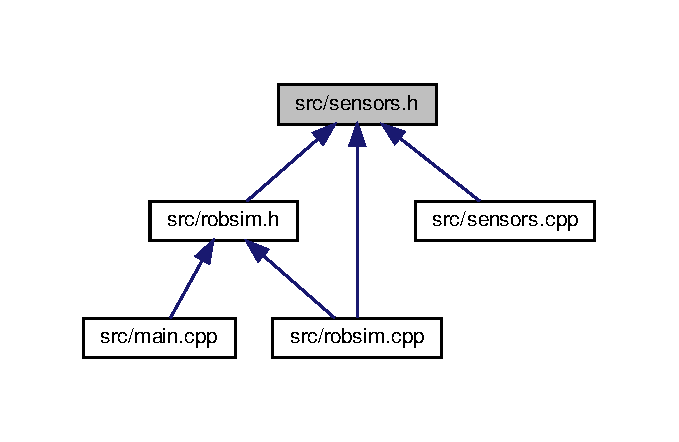
\includegraphics[width=326pt]{sensors_8h__dep__incl}
\end{center}
\end{figure}
\subsection*{Classes}
\begin{DoxyCompactItemize}
\item 
class \hyperlink{classMPU9250}{M\+P\+U9250}
\end{DoxyCompactItemize}

\hypertarget{timer_8h}{}\section{src/timer.h File Reference}
\label{timer_8h}\index{src/timer.\+h@{src/timer.\+h}}
{\ttfamily \#include $<$iostream$>$}\newline
{\ttfamily \#include $<$chrono$>$}\newline
{\ttfamily \#include $<$functional$>$}\newline
{\ttfamily \#include $<$thread$>$}\newline
Include dependency graph for timer.\+h\+:\nopagebreak
\begin{figure}[H]
\begin{center}
\leavevmode
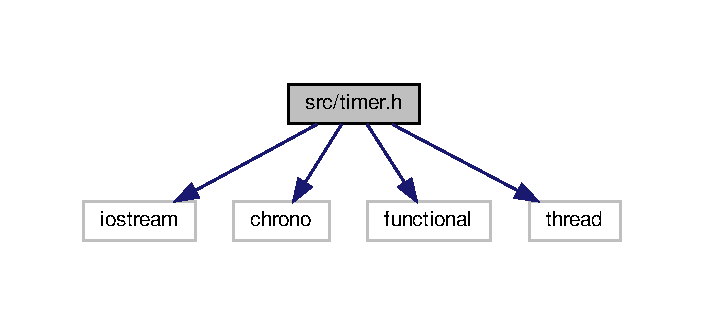
\includegraphics[width=338pt]{timer_8h__incl}
\end{center}
\end{figure}
This graph shows which files directly or indirectly include this file\+:\nopagebreak
\begin{figure}[H]
\begin{center}
\leavevmode
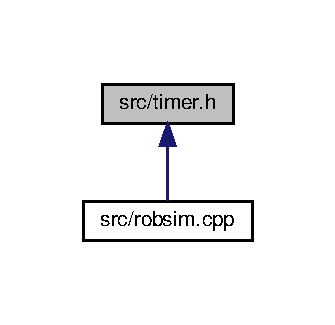
\includegraphics[width=161pt]{timer_8h__dep__incl}
\end{center}
\end{figure}
\subsection*{Classes}
\begin{DoxyCompactItemize}
\item 
class \hyperlink{classTimer}{Timer}
\begin{DoxyCompactList}\small\item\em Create asynchronous timers which execute specified functions in set time interval. \end{DoxyCompactList}\end{DoxyCompactItemize}

\hypertarget{utils_8cpp}{}\section{src/utils.cpp File Reference}
\label{utils_8cpp}\index{src/utils.\+cpp@{src/utils.\+cpp}}
{\ttfamily \#include $<$fstream$>$}\newline
{\ttfamily \#include $<$sstream$>$}\newline
{\ttfamily \#include $<$iostream$>$}\newline
{\ttfamily \#include \char`\"{}utils.\+h\char`\"{}}\newline
Include dependency graph for utils.\+cpp\+:\nopagebreak
\begin{figure}[H]
\begin{center}
\leavevmode
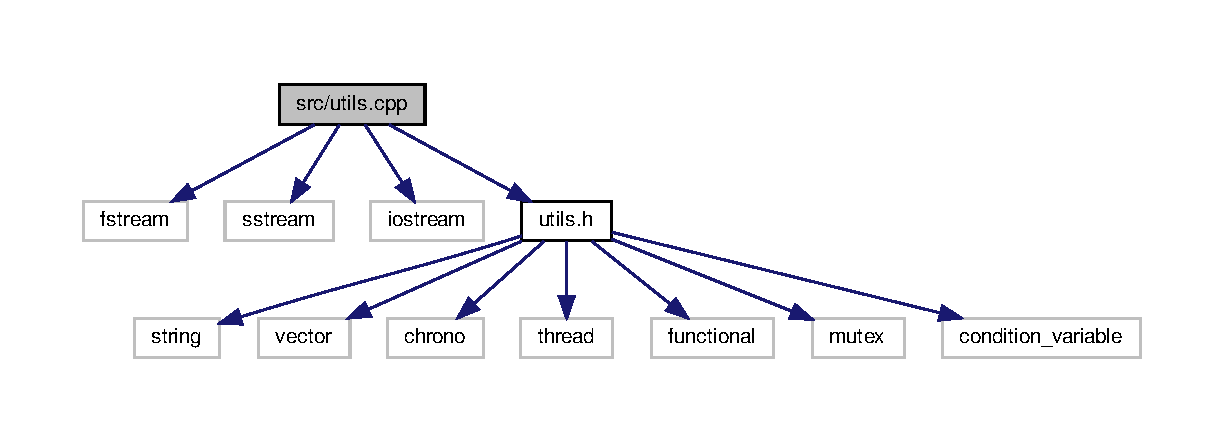
\includegraphics[width=350pt]{utils_8cpp__incl}
\end{center}
\end{figure}
\subsection*{Functions}
\begin{DoxyCompactItemize}
\item 
void \hyperlink{utils_8cpp_a1263999c182e68e204b84696cd247caa}{print\+\_\+end\+Menu} (void)
\item 
void \hyperlink{utils_8cpp_a94789c6523de64a6dda7f9b290bbd522}{print\+\_\+init\+Menu} (void)
\item 
vector$<$ vector$<$ double $>$ $>$ \hyperlink{utils_8cpp_ac026bb3b390444587a444a6b62655867}{Read\+\_\+\+C\+S\+V\+\_\+\+I\+M\+U\+\_\+\+C\+AM} (string input\+File\+Name)
\item 
string \hyperlink{utils_8cpp_ae1f0b848799389e13cbdedd8a79bde42}{decode\+\_\+msg} (string s, double v\mbox{[}3\mbox{]})
\end{DoxyCompactItemize}


\subsection{Function Documentation}
\mbox{\Hypertarget{utils_8cpp_ae1f0b848799389e13cbdedd8a79bde42}\label{utils_8cpp_ae1f0b848799389e13cbdedd8a79bde42}} 
\index{utils.\+cpp@{utils.\+cpp}!decode\+\_\+msg@{decode\+\_\+msg}}
\index{decode\+\_\+msg@{decode\+\_\+msg}!utils.\+cpp@{utils.\+cpp}}
\subsubsection{\texorpdfstring{decode\+\_\+msg()}{decode\_msg()}}
{\footnotesize\ttfamily string decode\+\_\+msg (\begin{DoxyParamCaption}\item[{string}]{s,  }\item[{double}]{v\mbox{[}3\mbox{]} }\end{DoxyParamCaption})}



Definition at line 85 of file utils.\+cpp.

\mbox{\Hypertarget{utils_8cpp_a1263999c182e68e204b84696cd247caa}\label{utils_8cpp_a1263999c182e68e204b84696cd247caa}} 
\index{utils.\+cpp@{utils.\+cpp}!print\+\_\+end\+Menu@{print\+\_\+end\+Menu}}
\index{print\+\_\+end\+Menu@{print\+\_\+end\+Menu}!utils.\+cpp@{utils.\+cpp}}
\subsubsection{\texorpdfstring{print\+\_\+end\+Menu()}{print\_endMenu()}}
{\footnotesize\ttfamily void print\+\_\+end\+Menu (\begin{DoxyParamCaption}\item[{void}]{ }\end{DoxyParamCaption})}



Definition at line 13 of file utils.\+cpp.

\mbox{\Hypertarget{utils_8cpp_a94789c6523de64a6dda7f9b290bbd522}\label{utils_8cpp_a94789c6523de64a6dda7f9b290bbd522}} 
\index{utils.\+cpp@{utils.\+cpp}!print\+\_\+init\+Menu@{print\+\_\+init\+Menu}}
\index{print\+\_\+init\+Menu@{print\+\_\+init\+Menu}!utils.\+cpp@{utils.\+cpp}}
\subsubsection{\texorpdfstring{print\+\_\+init\+Menu()}{print\_initMenu()}}
{\footnotesize\ttfamily void print\+\_\+init\+Menu (\begin{DoxyParamCaption}\item[{void}]{ }\end{DoxyParamCaption})}



Definition at line 26 of file utils.\+cpp.

\mbox{\Hypertarget{utils_8cpp_ac026bb3b390444587a444a6b62655867}\label{utils_8cpp_ac026bb3b390444587a444a6b62655867}} 
\index{utils.\+cpp@{utils.\+cpp}!Read\+\_\+\+C\+S\+V\+\_\+\+I\+M\+U\+\_\+\+C\+AM@{Read\+\_\+\+C\+S\+V\+\_\+\+I\+M\+U\+\_\+\+C\+AM}}
\index{Read\+\_\+\+C\+S\+V\+\_\+\+I\+M\+U\+\_\+\+C\+AM@{Read\+\_\+\+C\+S\+V\+\_\+\+I\+M\+U\+\_\+\+C\+AM}!utils.\+cpp@{utils.\+cpp}}
\subsubsection{\texorpdfstring{Read\+\_\+\+C\+S\+V\+\_\+\+I\+M\+U\+\_\+\+C\+A\+M()}{Read\_CSV\_IMU\_CAM()}}
{\footnotesize\ttfamily vector$<$vector$<$double$>$ $>$ Read\+\_\+\+C\+S\+V\+\_\+\+I\+M\+U\+\_\+\+C\+AM (\begin{DoxyParamCaption}\item[{string}]{input\+File\+Name }\end{DoxyParamCaption})}



Definition at line 44 of file utils.\+cpp.


\hypertarget{utils_8h}{}\section{src/utils.h File Reference}
\label{utils_8h}\index{src/utils.\+h@{src/utils.\+h}}
{\ttfamily \#include $<$string$>$}\newline
{\ttfamily \#include $<$vector$>$}\newline
{\ttfamily \#include $<$chrono$>$}\newline
{\ttfamily \#include $<$thread$>$}\newline
{\ttfamily \#include $<$functional$>$}\newline
{\ttfamily \#include $<$mutex$>$}\newline
{\ttfamily \#include $<$condition\+\_\+variable$>$}\newline
Include dependency graph for utils.\+h\+:\nopagebreak
\begin{figure}[H]
\begin{center}
\leavevmode
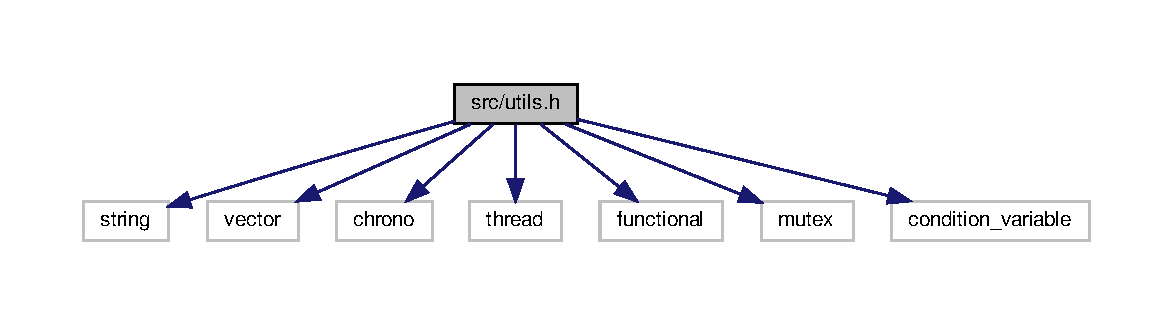
\includegraphics[width=350pt]{utils_8h__incl}
\end{center}
\end{figure}
This graph shows which files directly or indirectly include this file\+:\nopagebreak
\begin{figure}[H]
\begin{center}
\leavevmode
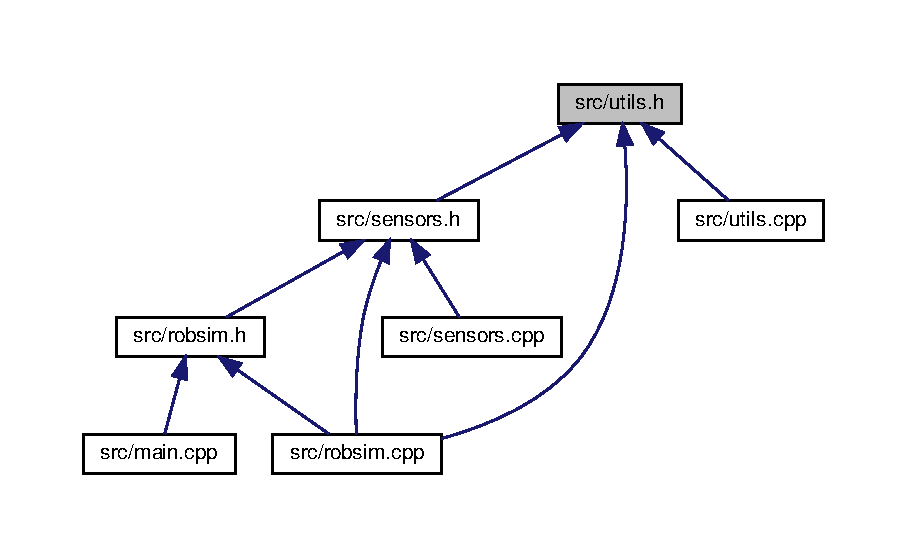
\includegraphics[width=350pt]{utils_8h__dep__incl}
\end{center}
\end{figure}
\subsection*{Macros}
\begin{DoxyCompactItemize}
\item 
\#define \hyperlink{utils_8h_ac0e2b53a3ea9ebce1dacd9413579ec69}{M\+S\+G\+\_\+\+D\+E\+L\+I\+M\+I\+T\+ER}~\char`\"{}\+:\char`\"{}
\item 
\#define \hyperlink{utils_8h_af392d7ee4f29a6a09970819dbd725c20}{M\+S\+G\+\_\+\+I\+MU}~\char`\"{}msg\+\_\+\+I\+MU\char`\"{}
\item 
\#define \hyperlink{utils_8h_a341cff82fa08399b66ed950cd301ffb6}{M\+S\+G\+\_\+\+C\+AM}~\char`\"{}msg\+\_\+\+C\+AM\char`\"{}
\item 
\#define \hyperlink{utils_8h_a43ca248958b3afe7f7c898a9e62b5a9c}{M\+S\+G\+\_\+\+B\+OM}~\char`\"{}msg\+\_\+\+B\+OM\char`\"{}
\item 
\#define \hyperlink{utils_8h_abf71abaffc4210c79acd651db9db90f8}{M\+S\+G\+\_\+\+L\+AS}~\char`\"{}msg\+\_\+\+L\+AS\char`\"{}
\end{DoxyCompactItemize}
\subsection*{Functions}
\begin{DoxyCompactItemize}
\item 
vector$<$ vector$<$ double $>$ $>$ \hyperlink{utils_8h_ac026bb3b390444587a444a6b62655867}{Read\+\_\+\+C\+S\+V\+\_\+\+I\+M\+U\+\_\+\+C\+AM} (string input\+File\+Name)
\item 
string \hyperlink{utils_8h_ae1f0b848799389e13cbdedd8a79bde42}{decode\+\_\+msg} (string s, double v\mbox{[}3\mbox{]})
\item 
void \hyperlink{utils_8h_a94789c6523de64a6dda7f9b290bbd522}{print\+\_\+init\+Menu} (void)
\item 
void \hyperlink{utils_8h_a1263999c182e68e204b84696cd247caa}{print\+\_\+end\+Menu} (void)
\end{DoxyCompactItemize}


\subsection{Macro Definition Documentation}
\mbox{\Hypertarget{utils_8h_a43ca248958b3afe7f7c898a9e62b5a9c}\label{utils_8h_a43ca248958b3afe7f7c898a9e62b5a9c}} 
\index{utils.\+h@{utils.\+h}!M\+S\+G\+\_\+\+B\+OM@{M\+S\+G\+\_\+\+B\+OM}}
\index{M\+S\+G\+\_\+\+B\+OM@{M\+S\+G\+\_\+\+B\+OM}!utils.\+h@{utils.\+h}}
\subsubsection{\texorpdfstring{M\+S\+G\+\_\+\+B\+OM}{MSG\_BOM}}
{\footnotesize\ttfamily \#define M\+S\+G\+\_\+\+B\+OM~\char`\"{}msg\+\_\+\+B\+OM\char`\"{}}



Definition at line 19 of file utils.\+h.

\mbox{\Hypertarget{utils_8h_a341cff82fa08399b66ed950cd301ffb6}\label{utils_8h_a341cff82fa08399b66ed950cd301ffb6}} 
\index{utils.\+h@{utils.\+h}!M\+S\+G\+\_\+\+C\+AM@{M\+S\+G\+\_\+\+C\+AM}}
\index{M\+S\+G\+\_\+\+C\+AM@{M\+S\+G\+\_\+\+C\+AM}!utils.\+h@{utils.\+h}}
\subsubsection{\texorpdfstring{M\+S\+G\+\_\+\+C\+AM}{MSG\_CAM}}
{\footnotesize\ttfamily \#define M\+S\+G\+\_\+\+C\+AM~\char`\"{}msg\+\_\+\+C\+AM\char`\"{}}



Definition at line 18 of file utils.\+h.

\mbox{\Hypertarget{utils_8h_ac0e2b53a3ea9ebce1dacd9413579ec69}\label{utils_8h_ac0e2b53a3ea9ebce1dacd9413579ec69}} 
\index{utils.\+h@{utils.\+h}!M\+S\+G\+\_\+\+D\+E\+L\+I\+M\+I\+T\+ER@{M\+S\+G\+\_\+\+D\+E\+L\+I\+M\+I\+T\+ER}}
\index{M\+S\+G\+\_\+\+D\+E\+L\+I\+M\+I\+T\+ER@{M\+S\+G\+\_\+\+D\+E\+L\+I\+M\+I\+T\+ER}!utils.\+h@{utils.\+h}}
\subsubsection{\texorpdfstring{M\+S\+G\+\_\+\+D\+E\+L\+I\+M\+I\+T\+ER}{MSG\_DELIMITER}}
{\footnotesize\ttfamily \#define M\+S\+G\+\_\+\+D\+E\+L\+I\+M\+I\+T\+ER~\char`\"{}\+:\char`\"{}}



Definition at line 16 of file utils.\+h.

\mbox{\Hypertarget{utils_8h_af392d7ee4f29a6a09970819dbd725c20}\label{utils_8h_af392d7ee4f29a6a09970819dbd725c20}} 
\index{utils.\+h@{utils.\+h}!M\+S\+G\+\_\+\+I\+MU@{M\+S\+G\+\_\+\+I\+MU}}
\index{M\+S\+G\+\_\+\+I\+MU@{M\+S\+G\+\_\+\+I\+MU}!utils.\+h@{utils.\+h}}
\subsubsection{\texorpdfstring{M\+S\+G\+\_\+\+I\+MU}{MSG\_IMU}}
{\footnotesize\ttfamily \#define M\+S\+G\+\_\+\+I\+MU~\char`\"{}msg\+\_\+\+I\+MU\char`\"{}}



Definition at line 17 of file utils.\+h.

\mbox{\Hypertarget{utils_8h_abf71abaffc4210c79acd651db9db90f8}\label{utils_8h_abf71abaffc4210c79acd651db9db90f8}} 
\index{utils.\+h@{utils.\+h}!M\+S\+G\+\_\+\+L\+AS@{M\+S\+G\+\_\+\+L\+AS}}
\index{M\+S\+G\+\_\+\+L\+AS@{M\+S\+G\+\_\+\+L\+AS}!utils.\+h@{utils.\+h}}
\subsubsection{\texorpdfstring{M\+S\+G\+\_\+\+L\+AS}{MSG\_LAS}}
{\footnotesize\ttfamily \#define M\+S\+G\+\_\+\+L\+AS~\char`\"{}msg\+\_\+\+L\+AS\char`\"{}}



Definition at line 20 of file utils.\+h.



\subsection{Function Documentation}
\mbox{\Hypertarget{utils_8h_ae1f0b848799389e13cbdedd8a79bde42}\label{utils_8h_ae1f0b848799389e13cbdedd8a79bde42}} 
\index{utils.\+h@{utils.\+h}!decode\+\_\+msg@{decode\+\_\+msg}}
\index{decode\+\_\+msg@{decode\+\_\+msg}!utils.\+h@{utils.\+h}}
\subsubsection{\texorpdfstring{decode\+\_\+msg()}{decode\_msg()}}
{\footnotesize\ttfamily string decode\+\_\+msg (\begin{DoxyParamCaption}\item[{string}]{s,  }\item[{double}]{v\mbox{[}3\mbox{]} }\end{DoxyParamCaption})}



Definition at line 85 of file utils.\+cpp.

\mbox{\Hypertarget{utils_8h_a1263999c182e68e204b84696cd247caa}\label{utils_8h_a1263999c182e68e204b84696cd247caa}} 
\index{utils.\+h@{utils.\+h}!print\+\_\+end\+Menu@{print\+\_\+end\+Menu}}
\index{print\+\_\+end\+Menu@{print\+\_\+end\+Menu}!utils.\+h@{utils.\+h}}
\subsubsection{\texorpdfstring{print\+\_\+end\+Menu()}{print\_endMenu()}}
{\footnotesize\ttfamily void print\+\_\+end\+Menu (\begin{DoxyParamCaption}\item[{void}]{ }\end{DoxyParamCaption})}



Definition at line 13 of file utils.\+cpp.

\mbox{\Hypertarget{utils_8h_a94789c6523de64a6dda7f9b290bbd522}\label{utils_8h_a94789c6523de64a6dda7f9b290bbd522}} 
\index{utils.\+h@{utils.\+h}!print\+\_\+init\+Menu@{print\+\_\+init\+Menu}}
\index{print\+\_\+init\+Menu@{print\+\_\+init\+Menu}!utils.\+h@{utils.\+h}}
\subsubsection{\texorpdfstring{print\+\_\+init\+Menu()}{print\_initMenu()}}
{\footnotesize\ttfamily void print\+\_\+init\+Menu (\begin{DoxyParamCaption}\item[{void}]{ }\end{DoxyParamCaption})}



Definition at line 26 of file utils.\+cpp.

\mbox{\Hypertarget{utils_8h_ac026bb3b390444587a444a6b62655867}\label{utils_8h_ac026bb3b390444587a444a6b62655867}} 
\index{utils.\+h@{utils.\+h}!Read\+\_\+\+C\+S\+V\+\_\+\+I\+M\+U\+\_\+\+C\+AM@{Read\+\_\+\+C\+S\+V\+\_\+\+I\+M\+U\+\_\+\+C\+AM}}
\index{Read\+\_\+\+C\+S\+V\+\_\+\+I\+M\+U\+\_\+\+C\+AM@{Read\+\_\+\+C\+S\+V\+\_\+\+I\+M\+U\+\_\+\+C\+AM}!utils.\+h@{utils.\+h}}
\subsubsection{\texorpdfstring{Read\+\_\+\+C\+S\+V\+\_\+\+I\+M\+U\+\_\+\+C\+A\+M()}{Read\_CSV\_IMU\_CAM()}}
{\footnotesize\ttfamily vector$<$vector$<$double$>$ $>$ Read\+\_\+\+C\+S\+V\+\_\+\+I\+M\+U\+\_\+\+C\+AM (\begin{DoxyParamCaption}\item[{string}]{input\+File\+Name }\end{DoxyParamCaption})}



Definition at line 44 of file utils.\+cpp.


%--- End generated contents ---

% Index
\backmatter
\newpage
\phantomsection
\clearemptydoublepage
\addcontentsline{toc}{chapter}{Index}
\printindex

\end{document}
